\documentclass[usenatbib,fleqn]{mnras}
\pdfoutput=1 %for arxiv
\setlength{\topmargin}{-0.3in}
\usepackage{amssymb}
\usepackage{amsmath}
\usepackage[dvipsnames]{xcolor}  
\usepackage{graphicx}
\usepackage[T1]{fontenc}
\usepackage{newtxtext,newtxmath}
\usepackage[figure,figure*]{hypcap}
%Journals
\def\pasj{{PASJ}}
\def\nat{{ Nature }}
\def\aap{{ Astron. \& Astrophys. }}
\def\aj{{ Astron.~J. }}
\def\apj{{ Astrophys.~J. }}
\def\araa{{ Ann. Rev. Astron. Astrophys. }}
\def\apjl{{ Astrophys.~J.~Letters }}
\def\apjs{{ Astrophys.~J.~Suppl. }}
\def\apss{{ Astrophys.~Space~Sci. }}
\def\icarus{{ Icarus }}
\def\mnras{{ MNRAS }}
\def\pasp{{ Pub. Astron. Soc. Pacific }}
\def\planss{{ Plan. Space Sci. }}
\def\physrep{{ Phys. Rep.}}
\def\jcap{{J. Cosm. Astropart. Phys.}}

% less then similar, greater than similar
\def\lsim{\lower0.6ex\vbox{\hbox{$ \buildrel{\textstyle <}\over{\sim}\ $}}}
\def\gsim{\lower0.6ex\vbox{\hbox{$ \buildrel{\textstyle >}\over{\sim}\ $}}}

% begin equation
\newcommand{\beq}{\begin{equation}}
\newcommand{\eeq}{\end{equation}}
\newcommand{\beqa}{\begin{eqnarray}}
\newcommand{\eeqa}{\end{eqnarray}}

% basic cosmology
\newcommand{\Ho}{H_{0}}
\newcommand{\Om}{\Omega_{\mathrm{M}}}
\newcommand{\Ol}{\Omega_{\Lambda}}
\newcommand{\Ode}{\Omega_{\mathrm{DE}}}
\newcommand{\rhocrit}{\rho_{\mathrm{crit}}}
\newcommand{\Ok}{\Omega_{\mathrm{K}}}
\newcommand{\wzero}{w_{0}}
\newcommand{\wa}{w_{\mathrm{a}}}
\newcommand{\wpiv}{w_{\mathrm{piv}}}
\newcommand{\apiv}{a_{\mathrm{piv}}}
\newcommand{\ellmax}{\ell_{\mathrm{max}}}
\newcommand{\fsky}{f_{\mathrm{sky}}}

\newcommand{\fom}{\mathcal{F}}
\newcommand{\Rvir}{r_{\mathrm{vir}}}
\newcommand{\Rdel}{r_{\Delta}}

% units
\newcommand{\Msun}{\mathrm{M}_{\odot}~}
\newcommand{\hMsun}{\ h^{-1}\mathrm{M}_{\odot}~}
\newcommand{\hMpc}{\ h^{-1}\mathrm{Mpc}~}
\newcommand{\hkpc}{\ h^{-1}\mathrm{kpc}~}
\newcommand{\cpiv}{c_{\mathrm{piv}}}
\newcommand{\kmsmpc}{~\mathrm{km/s/Mpc}~}
\newcommand{\kms}{~\mathrm{km}~\mathrm{s}^{-1}}
\newcommand{\Mpc}{\mathrm{Mpc}}
\newcommand{\kpc}{\mathrm{kpc}}
\newcommand{\pc}{\mathrm{pc}}
\newcommand{\au}{\mathrm{AU}}
\newcommand{\gev}{\mathrm{GeV}}

% roman differential
%\newcommand{\dd}{\mathrm{d}}

% comments
\newcommand{\arz}[1]{{\color{BrickRed}\textbf{[ARZ: }\textbf{#1}]}}


% attempt stolen from Google to try to fix figure pileup.
\renewcommand{\topfraction}{.85}
\renewcommand{\bottomfraction}{.7}
\renewcommand{\textfraction}{.15}
\renewcommand{\floatpagefraction}{.66}
\renewcommand{\dbltopfraction}{.66}
\renewcommand{\dblfloatpagefraction}{.66}
\setcounter{topnumber}{9}
\setcounter{bottomnumber}{9}
\setcounter{totalnumber}{20}
\setcounter{dbltopnumber}{9}
%%%%%%%%%%%%%%%%%%%%%%%%%%%%%%%%%%%%%%%%%%%%%%%%

\title[The Immitigable Nature of Assembly Bias]{The Immitigable Nature of Assembly
Bias: the Impact of Halo Definition on Environmental Effects}
\author[A.~S.~Villarreal et al.]{%
Antonio~S.~Villarreal$^{1}$\thanks{E-mail: \email{asv13@pitt.edu}},
Andrew~R.~Zentner$^{1}$\thanks{E-mail: \email{zentner@pitt.edu}},
Yao-Yuan~Mao$^{1}$, %\thanks{E-mail: yymao@pitt.edu}
Chris~W.~Purcell$^{2}$,%\thanks{E-mail: cwpsps@rit.edu}
\newauthor
Andrew~P.~Hearin$^{3}$, %\thanks{E-mail: andrew.hearin@yale.edu}
Frank~C.~van~den~Bosch$^{3}$, %\thanks{E-mail: frank.vandenbosch@yale.edu} 
Benedikt~Diemer$^{4}$, %\thanks{E-mail: benedikt.diemer@cfa.harvard.edu}
Johannes~U.~Lange$^{3}$,
\newauthor
and Kuan~Wang$^{1}$
\\
$^{1}$Department of Physics and Astronomy \& Pittsburgh Particle Physics, Astrophysics, and Cosmology Center (Pitt-PACC), \\
\phantom{$^{1}$}University of Pittsburgh, Pittsburgh, PA\\
$^{2}$School of Physics and Astronomy \& Center for Computational Relativity and Gravitation (CCRG), Rochester Institute of Technology, Rochester, NY \\
$^{3}$Department of Astronomy, Yale University, Hew Haven, CT\\
$^{4}$Center for Astrophysics, Harvard University, Cambridge, MA}

\pubyear{2017}

%% to allow it to compile until we find where the link problem is
%% and fix with clever wording.
%% \hypersetup{draft}
\begin{document}
\label{firstpage}
\pagerange{\pageref{firstpage}--\pageref{lastpage}} 

\maketitle

\begin{abstract}
%% Abstract goes here

Dark matter halos cluster in a manner that depends upon halo mass, but 
also upon other halo properties such as concentration and shape. This is known broadly as {\em assembly bias}. This poses a challenge to phenomenological models of galaxy clustering that assume that galaxies may be mapped onto halos as a function of halo mass alone. We explore the strength of assembly bias as a function of the definition of the halo, parameterized by the spherical overdensity, $\Delta$. In agreement with 
previous studies, we find that concentration-dependent clustering 
depends strongly upon halo mass. We find that the strength and 
even the sense of halo assembly bias depends significantly upon halo 
definitions, varying by as much as $\sim 50\%$ among common definitions. 
Concentration dependent clustering can be greatly reduced by adopting a mass-dependent halo definition because such a definition assigns so-called 
{\em splashback} halos as satellite halos of a now, larger, host halo. However, the halo definitions that best mitigate concentration dependent halo clustering do not coincide with halos defined by their splashback radii. Shape and spin dependent clustering are present at similar levels for all halo definitions that we explore. Further studies are necessary 
to develop models that may be used to interpret high-precision data.

\end{abstract}

\begin{keywords}
cosmology: dark matter -- cosmology: large-scale structure of Universe -- galaxies: formation -- galaxies: haloes -- methods: numerical
\end{keywords}

%% notes on citation style:
%% \citep{stuff01,stuff02,stuff03} produces (Stuff 2001; Stuff 2002; Stuff 2003)
%% \citet{stuff04} produces ``Stuff (2004)'' in the main body
%% \\* defines a break in a section title it appears?
%% \begin{enumerate} into \item allows you to do the (i), (ii), (iii) thing 


%-----------------------
\section{Introduction}
\label{section:introduction}
%-----------------------

In the concordance cosmology, galaxies and clusters form within dark matter halos \citep{white_rees78,blumenthal_etal84, mo_etal10}. Numerical simulations have provided a solid understanding of the abundances, properties, and clustering of dark matter halos. Accordingly, it is possible to compute the clustering statistics of galaxies given a model for the relationship between galaxies and dark matter halos. 
Such halo occupation models have been used to interpret large-scale structure measurements and 
constrain models of galaxy evolution \citep{yang_etal03,tinker_etal05,zehavi_etal05b,porciani_norberg06,vdbosch_etal07,zheng_etal07,conroy_wechsler09,
yang_etal09b,zehavi_etal11,guo_etal11a,wake_etal11,yang_etal11a,yang_etal12,leauthaud_etal12,
rodriguezpuebla_etal12, behroozi_etal13b, moster_etal13, tinker_etal13,cacciato_etal13,more_etal13,guo_etal14,
zu_mandelbaum15b}.
To date, the vast majority of halo occupation models rely on a key assumption, namely that the probability of a halo to host a number of galaxies of a particular type depends only upon halo mass. It is now well known that the clustering strength of halos depends upon properties such as halo formation time \citep{gao_etal05,harker_etal06, wechsler_etal06,gao_white07,croton_etal07,zentner07,dalal_etal08, li_etal08, lacerna_padilla11}, concentration \citep{wechsler_etal06,faltenbacher_white10, mao_etal15}, and other halo properties \citep{bett_etal07, hahn_etal07a, hahn_etal07b, faltenbacher_white10, vandaalen_etal12, fisher_faltenbacher16, sunayama_etal16, chavesmontero_etal16}. If galaxy properties depend upon these halo properties, a phenomenon known as galaxy {\em assembly bias}, then standard halo occupation modelling will fail \citep{zentner_etal14} and more complex models \citep{gilmarin_etal11, hearin_etal16} will be necessary.

\arz{Antonio - can you please self-consistently add the citations to 
Miyatake et al. 16, More et al. 16, Zu et al. 16, Lehmann et al. 17, Hearin et al. 16, and Zentner et al. 16 to this paragraph. 
Frank or Andrew H. may want to a bit about conformity studies?}
There exist some hints of assembly bias in the literature. \citet{miyatake_etal16} and \citet{more_etal16} presented 
evidence that clusters with more centrally-concentrated 
satellite galaxy distributions cluster more weakly than 
their less centrally-concentrated counterparts 
\citep[however][demonstrate that this claim is likely to be 
compromised by environment-dependent cluster membership assignment]{zu_mandelbaum16}. \citet{lehmann_etal17} demonstrated that observed galaxy 
clustering can be more well-described by models in which galaxy 
stellar mass depends upon halo concentration as well as halo mass. 
Using decorated halo occupation distribution (HOD) models \citep{hearin_etal16}, \citet{zentner_etal16} interpreted observed 
galaxy clustering in the context of models that include assembly bias 
finding marginal evidence that halo occupation depends upon both halo mass and halo concentration. These findings suggest that assembly bias is 
important to consider when interpreting galaxy clustering and that assembly bias may be critical to the interpretation of forthcoming, 
higher-precision data sets.

In this work, we explore the possibility of simplifying halo occupation modelling, at least for some applications, by altering the definition of the boundary of a halo. Though motivated broadly by spherical collapse \citep{gunn_gott72, fillmore_goldreich84, ryden_gunn87, lacey_cole93, eke_etal96, mota_vandebruck04, pace_etal10}, specific halo definitions have become a matter of convention that vary considerably in the literature. Many authors define halos using a friends-of-friend (FoF) algorithm applied to the particle distribution \citep[e.g., ][]{davis_etal85}. More often, authors define halos by spherical overdensity (SO) regions within which the mean density exceeds a particular threshold \citep[e.g., ][]{lacey_cole93}. These halo definitions are reviewed in \citet[][and references therein]{knebe_etal11}. The threshold used varies significantly. With respect to the mean density of the universe, commonly used thresholds are 178, 180, 200, and $\sim$340 times the mean background density, motivated by spherical collapse models for different cosmologies. Many authors define halos by an overdensity of 200 with respect to the critical density of the universe, motivated as an approximation to the virial radius at high redshift. This corresponds to $\Delta \approx 625$ with respect to the mean density in a concordance cosmological model. Significantly higher values of the overdensity parameter are often used in studies of X-ray emission from cluster-sized halos, where observations only cover large overdensities and correspondingly small radii.

We study the strength of various halo assembly bias signals as a function of halo definition. To be specific, we restrict ourselves to halos that are defined by spherical regions and we study the strength of halo assembly bias as a function of the density threshold used to demarcate these halos. This is motivated, in large part, by recent literature suggesting that a large portion of assembly bias stems from halos in the relatively dense environments surrounding larger halos \citep{wang_etal07,warnick_etal08,more_etal15,sunayama_etal16}. The picture is that interactions with a relatively small number of large halos influence the evolution and structural properties of nearby, smaller halos. Indeed, the environmental impacts of halos on one another has been shown to extend beyond well beyond traditional 
virial radii \citep{wetzel_etal14,diemer_kravtsov14,behroozi_etal13b,adhikari_etal14,wetzel_nagai15,more_etal15}. Halos in dense environments (e.g., near other large halos) exhibit anomalous properties (e.g., formation times, concentrations, shapes) compared to field halos in part because of their interactions with their larger, neighbours. It seems interesting to ask whether or not a halo definition in which large halos contain many of these smaller, anomalous neighbour halos can mitigate halo assembly bias. In this way, the halo boundary may serve as a more meaningful boundary around regions within which highly nonlinear effects are important. Assessing this strategy is the aim of our paper. 

We conclude that alternative halo definitions do {\em not} generally mitigate halo assembly bias for two reasons. First, no single halo definition mitigates all forms of halo assembly bias. For example, a halo definition that mitigates concentration-based halo clustering does not simultaneously mitigate angular momentum-dependent halo clustering. Second, any halo definition that mitigates any form  of assembly bias must be strongly mass dependence, adding a great deal of complexity to halo finding. The details of our work have other interesting implications. Perhaps most importantly, our work emphasizes the fact that halo assembly bias effects are strongly dependent upon halo definitions. Therefore, one must exercise care in comparing the work of different authors who may have used different halo definitions. Our final results summarizes halo assembly bias as a function of halo definition.
 
In \S~\ref{section:data} of this paper, we discuss the cosmological simulations and halo finders utilized in the analysis. In \S~\ref{section:haloprops}, we discuss and define the halo properties used as our tracers of assembly bias. In \S~\ref{section:methodology}, we discuss the statistics that we use to measure environmental effects after halo redefinition. We also discuss our method of removing known mass scaling from halo properties. In \S~\ref{section:results}, we present our findings and consider how the change of halo definition impacts measures of assembly bias. In \S~\ref{section:conclusions}, we discuss the significance of our results in the context of halo modelling. We also consider the nature of assembly bias as a function of halo definition.

%------------------------------------
\section[]{Simulations and Halo Identification}
\label{section:data}
%------------------------------------


In order to study the effects of halo redefinition, we use three cosmological $N$-body simulations of structure formation. These simulations are a subset of the  \citet{diemer_kravtsov15} simulations performed within the Planck best-fit cosmology with $\Om = 0.32$, $\Ol = 0.68$, and $h_0 = 0.67$. We use three simulation boxes with comoving box lengths of 125, 250, and 500$\hMpc$ respectively. Each simulation models the evolution of $1024^3$ particles implying particle masses of $1.6 \times 10^8$, $1.3 \times 10^9$, and $1.0 \times 10^{10}\hMsun$ respectively. The three simulations have force softening scales of $2.4$, $5.8$, and $14 \hkpc$. We refer to each simulation as
\simA, \simB, or \simC~ for the remainder of the paper. This set of simulations allows us to probe the resolution effects and to probe the mass dependence of halo clustering over a wider range of halo masses than would be possible with only one simulation from the set. For example, \simA, with its higher resolution, contains the least massive resolved halos, while \simC~has a larger number of high-mass halos.

To identify halos, we use the {\tt ROCKSTAR} halo finder, which works on the phase space algorithm described in \citet*{behroozi_etal13a}. In short, {\tt ROCKSTAR} determines initial groupings of particles using a Friends-of-Friends algorithm in phase space before applying the spherical overdensity halo definition in order to calculate halo properties of interest. Unbound particles are removed prior to the calculation of halo mass and other halo properties. Our method of halo redefinition is to change how halo size is calculated as part of the {\tt ROCKSTAR} pipeline. A halo is given a radius, $\Rdel$, determined by
\beq
	\bar{\rho}(\Rdel) = \Delta \rho_{\mathrm{m}}, 
\eeq
where the mean density within a spherical volume of radius $r$ is $\bar{\rho}(r)$, $\Delta$ is the overdensity parameter, and $\rho_{\mathrm{m}}$ is the mean background mass density of the simulation. The resulting halo radius can vary widely dependent upon the choice of $\Delta$. \footnote{It is worth noting that the {\tt ROCKSTAR} linking length parameter must be adjusted as $\Delta$ varies in order to ensure that SO halos contain all relevant particles. The value we choose ($0.4$) is large enough that it works for all definitions.} The number chosen for $\Delta$ varies throughout the literature from $\Delta \approx 178$ to $\Delta \approx 340$. Many authors define halos as an overdensity of $\approx 200$ with respect to the critical density, which corresponds to an overdensity with respect to the mean density of $\Delta \approx 625$. X-ray studies of clusters use higher overdensities to isolate the regions within which they have data, with overdensities reaching as high as $\Delta \approx 7800$ (an overdensity with respect to the critical density of $\approx 2500$). 

We vary the sizes of a halos by treating the overdensity parameter as tunable, and our most interesting results correspond to values from $\Delta \approx 20$ to $\Delta \approx 625$, which spans the range used in the literature on galaxy clustering. 
The impact of the choice of $\Delta$ on halo radius and halo size can be seen in Figure \ref{fig:deltacompare}.

\begin{figure}
\centering
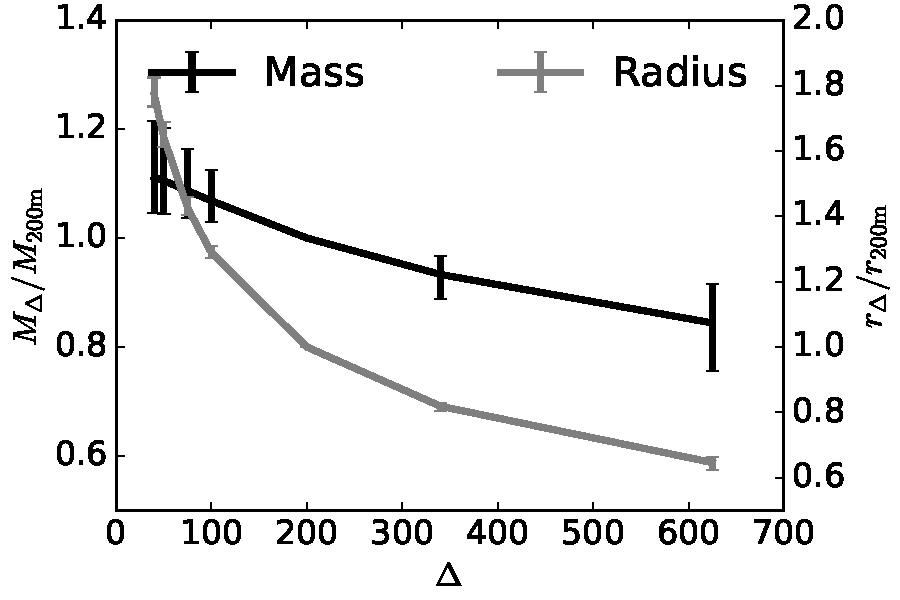
\includegraphics[width=\columnwidth]{massvsdelta_l0250.pdf}
\caption{
The ratio of halo properties as a function of $\Delta$ in the \simB~ catalog. The sample contains all host halos with masses greater than $M_{200\mathrm{m}} \ge 7.1 \times 10^{11}$. The black (dark grey) line shows the median value of the ratio of the halo mass (halo radius) at a value of $\Delta$ to the value at $\Delta=200\mathrm{m}$. The error bars contain 68\% of values of this ratio for the sample. These ratios are 
very mild functions of mass, but all masses are stacked in this plot.}
\label{fig:deltacompare}
\end{figure}

The {\tt ROCKSTAR} software also effectively identifies halo substructure, commonly referred to in the literature as subhalos. All density peaks are identified within the simulation and if a halo exists within the phase space of another halo, the less massive of the two is defined to be a subhalo of the more massive companion. The more massive companion is referred to as the host halo. This process continues until all halos identified in the simulation have been designated as either host halos or subhalos.

%-------------------------------------
\section{Halo Properties}
\label{section:haloprops}
%-------------------------------------

As has long been well known, halo mass is the property that most strongly affects halo clustering. In this paper, we aim to study the strength of halo clustering as a function of halo properties other than mass. We will refer to these properties as ``auxiliary'' halo properties in this paper. Throughout the remainder of the paper, we refer to halo two-point clustering that depends upon one of these auxiliary properties at fixed mass variously as ``halo assembly bias,'' ``auxiliary property dependent'' clustering, or simply ``environmental dependence'' of the auxiliary property. The properties we study are described in this section.

%----------------------------------------
\subsection{Measures of Halo Concentration}

We investigate halo clustering as a function of two definitions of halo concentration. The first stems from a fit of the spherically-averaged halo density profile, $\rho(r)$, to a \citet{navarro_etal97} (hereafter, NFW) density profile, 
%
\beq
\rho(r) = \frac{\rho_0}{\frac{r}{r_{\mathrm{s}}}\left(1+\frac{r}{r_{\mathrm{s}}}\right)^2},
\eeq
%
where the density scale, $\rho_0$, and the scale radius, $r_{\mathrm{s}}$, are parameters that are fit to the density profile of each halo. The standard definition of halo concentration is then 
\beq
c_{\mathrm{NFW}} = \frac{\Rdel}{r_\mathrm{s}},
\eeq
where $\Rdel$ is the radius of the halo given an overdensity parameter, $\Delta$, defining the halo and $r_{\mathrm{s}}$ is the inferred halo scale radius. We use the NFW concentrations computed by the {\tt ROCKSTAR} halo finder, which are derived from a fit to the halo density profile.  


The NFW concentration defined in the previous paragraph has the shortcoming that it 
depends upon a parametric description of dark matter halos, so we study the clustering dependence of halos as a function of a non-parametric description of halo concentration as well. In particular, we use the ``velocity-ratio'' concentration \citep{prada_etal12,klypin_etal16},
\beq
c_{\mathrm{V}} = \frac{V_{\mathrm{max}}}{V_{\Delta}}, 
\eeq
where $V_{\mathrm{max}}$ is the maximum circular velocity achieved within the halo and $V_{\Delta}$ is the circular velocity at the halo radius, $\Rdel$. All halos of the same mass have the same value of $V_{\Delta}$; however, 
they exhibit a variety of $V_{\mathrm{max}}$ values depending upon the degree to which their masses are concentrated toward the halo center. The quantity $c_{\mathrm{V}}$ is a non-parametric measure of halo concentration and can be measured from simulation snapshots without fitting halo density profiles. Consequently, $c_{\mathrm{V}}$ is robust to halo density profile parametrizations and halo profile fitting procedures. 

Halo concentrations are interesting to investigate for these purposes for a number of reasons. First of all, the environment dependence of halo concentrations is known to be strong for standard halo definitions. Second, halo concentrations are of interest in the modelling of galaxy clustering and gravitational lensing statistics (and their cross correlations). In the case of galaxy clustering, the relevance is indirect, because galaxies may not trace the mass densities of their host halos. In the case of gravitational lensing, the mass distribution is the primary quantity of interest and halo concentrations are directly related to predictions for lensing statistics. 

A third motivation to study halo concentrations is that halo concentrations are known to be strongly correlated with the formation histories of dark matter halos with earlier forming halos having higher concentrations at fixed halo mass \citep{wechsler_etal02, zhao_etal03, wechsler_etal06, zhao_etal09}. 
As such, exploring the concentration dependence of halo clustering may yield insight into the age dependence of halo clustering without the need for constructing merger trees. This is particularly important for our study in which the halo finding is performed repeatedly for many different values of $\Delta$. Constructing a self-consistent merger tree from which halo formation history can be 
studied requires halo finding at all simulation snapshots for each new value of $\Delta$, which is a computationally prohibitive task. In the present paper, we limit our study to halo properties that can be measured from a single simulation 
snapshot. 

A note of caution regarding the previous discussion is that halo formation histories correlate with halo concentrations with significant scatter and this correlation may depend upon environment, so the reader must be wary of drawing conclusions about the environmental dependence of halo formation by extrapolating our results on halo concentration. We will explore measures of halo age directly in a forthcoming follow-up study dedicated to halo formation histories.

Figure~\ref{fig:massrelation} shows the mean $c_{\mathrm{NFW}}$-$M_{\Delta}$ relation for halos defined with $\Delta=200$ in \simA, \simB, and \simC. For each simulation, we consider halos only above a minimum mass threshold to ensure that property measurements are not compromised by resolution effects. The minimum mass thresholds are shown as the vertical lines in Fig.~\ref{fig:massrelation} and listed in Table~\ref{table:thresholds} alongside the associated minimum number of particles. Figure~\ref{fig:massrelation} also shows the relation between the velocity-ratio concentration, $c_{\mathrm{V}}$, and halo mass. In the interest of completeness, Figure~\ref{fig:concentrations} shows the relationship 
between $c_{\mathrm{NFW}}$ and $c_{\mathrm{V}}$ on a halo-by-halo basis. As is evident, the two concentration proxies are strongly correlated and exhibit a $\sim 6\%$ scatter indicating that $c_{\mathrm{NFW}}$ and $c_{\mathrm{V}}$ indeed encode similar information about each halo.

%------------------------------------------ Figure for Cnfw(M)
\begin{figure*}
\centering
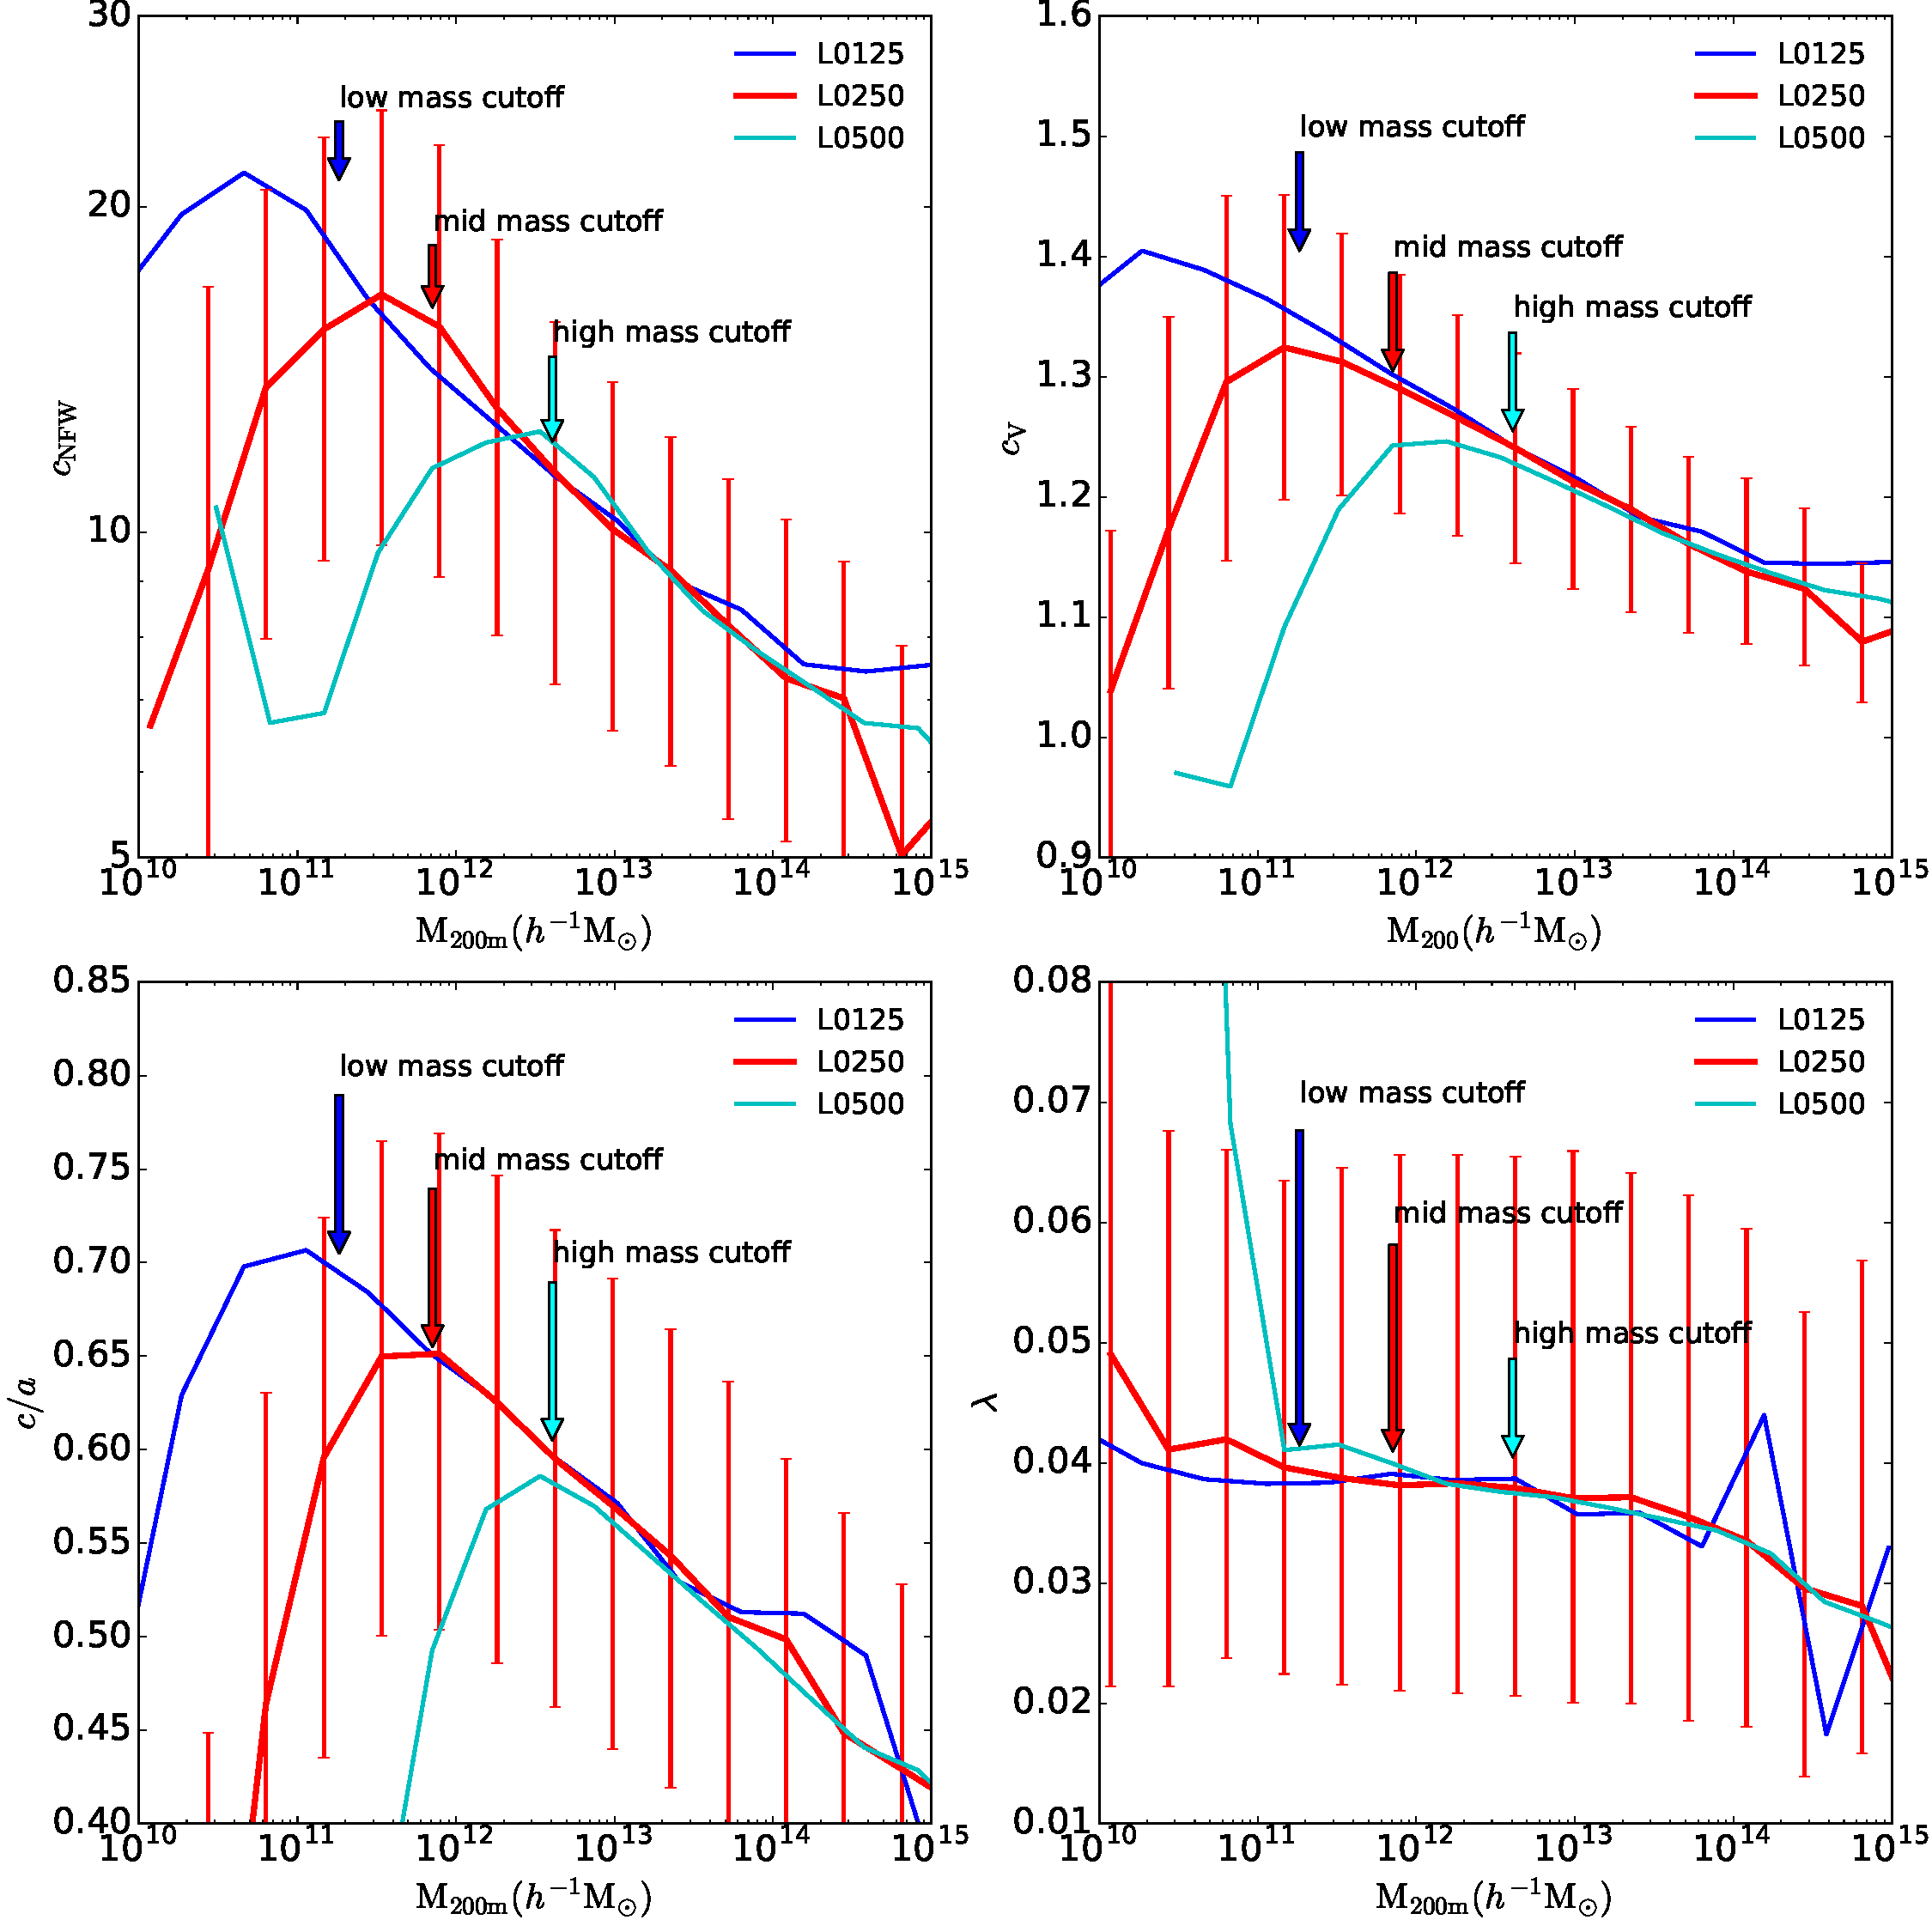
\includegraphics[width=\textwidth]{masscuts_d200.pdf}
\caption{
The relationship between halo properties and halo mass for each of our simulations with $\Delta =200$. These properties are the halo NFW-defined concentration, the velocity ratio defined concentration, the halo shape, and the halo spin. In order of increasing simulation volume, the blue line corresponds to the concentration-mass relation from simulation \simA, the red line corresponds to \simB, and the cyan line corresponds to \simC. The red error bars show the 68\% spread in parameter values within that mass bin for \simB. These errors are comparable to those of the other simulations within the region of interest. Each simulation is subject to resolution limitations at different halo masses. We show with arrows the minimum $M_{200}$ mass thresholds that we adopt in our analyses using the same colour code as the concentration-mass relations, going from \simA \ to \simC \ from left to right. Note the deviation from monotonic trends as a result of resolution effects.
}
\label{fig:massrelation}
\end{figure*}
%--------------------------------------------------------------------------------



%-------------------------------------------- Figure comparing Cnfw and Cv on a halo-by-halo basis
\begin{figure}
\centering
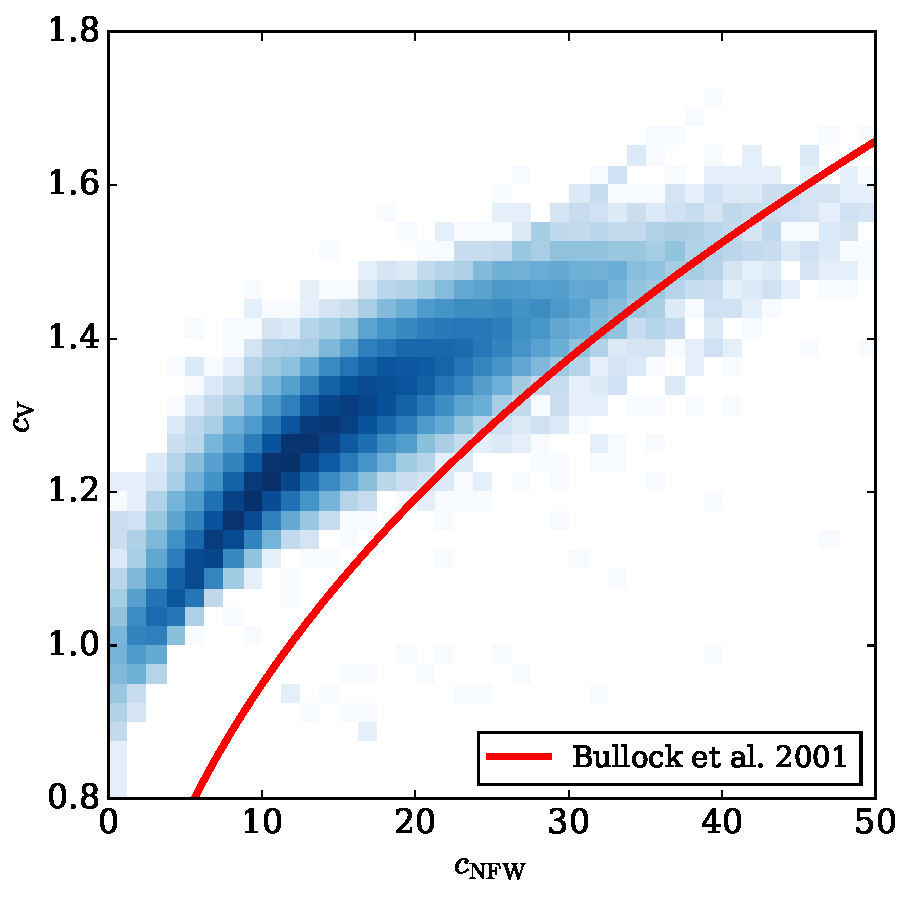
\includegraphics[width=\columnwidth]{cvvscnfw_relation.pdf}
\caption{
The relationship between the two different measures of concentration, 
using halos in \simB. The colour scale, shown at the right, encodes the number of halos within a single two-dimensional bin in the $c_{\mathrm{NFW}}$-$c_{\mathrm{V}}$ space. The red (blue) regions on the plot show where the most (fewest) halos exist with those values of the two concentration parameters. The white regions indicate where no halos hold these values. The scatter on this relationship ranges from 5\% for intermediate concentration values, to a high of 13\% at high masses.
}
\label{fig:concentrations}
\end{figure}
%--------------------------------------------------------------------------------------------------------------------------------


%---------------------------------------
\subsection{Halo Shape}

In addition to halo concentrations, we examine halo clustering as a function of a variety of other halo properties. We study halo clustering as a function of halo shape, $s$, quantified by the ratio of the halo minor, $c$ and major, $a$, axis lengths, 
%
\beq
s = \frac{c}{a}.
\eeq
%
The halo shapes we used were measured with {\tt ROCKSTAR} by calculating the mass distribution tensor,
\beq
M_{ij}=\frac{1}{N}\sum\limits_{N}\frac{x_i x_j}{r_{ij}^2},
\eeq
for all particles within the halo radius, including particles associated with identified substructure, where $x_i$ is the position from the halo center along a given axis and $r_{ij}$ is the distance between the particle and the halo center and weights the overall calculation. The sorted eigenvalues of the matrix represent the squares of the principal ellipsoid axes, where $a > b > c$. The mean relations for halo shapes as a function of halo mass for $\Delta=200$ are shown in Figure~\ref{fig:massrelation} along with the mass thresholds used to ensure that our results are not compromised by 
resolution.


%-----------------------------
\subsection{Halo Spin}

We study halo clustering as a function of halo angular momentum quantified 
by the spin parameter, $\lambda$, as introduced by \citep{peebles69},
\beq
\lambda = \frac{J \sqrt{\lvert E\rvert}}{G M_{\Delta}^{2.5}}
\eeq
where $J$ is the halo angular momentum, $E$ is the total energy of the 
halo, and $M_{\Delta}$ is the mass at the halo radius, $r_{\Delta}$. We measure this quantity using {\tt ROCKSTAR} which calculates the angular momentum, total energy, and total mass within $\Delta$ using bound particles out to the corresponding halo radius.
The mean relations for halo spin as a function of halo mass for $\Delta=200$ are shown in Figure~\ref{fig:massrelation} along with the mass thresholds enforced to ensure that our results are not compromised by resolution. These thresholds are summarized in Table~\ref{table:thresholds}, where we also show the threshold masses at various values of the overdensity parameter, $\Delta$.

%---------------------------------
\subsection{Halo Samples}

In practice, the mean relations between the various halo properties and the mass 
thresholds for our analyses must be determined separately for each combination of simulation, halo property (e.g., $c_{\mathrm{NFW}}$ or $s$), and halo definition (i.e., value of $\Delta$ in the case of the present study). For each analysis, we set mass thresholds in order to avoid the regime in which halo parameters are not well measured due to resolution limits of the simulations; we draw attention to the deviation in the upper-right panel of Figure~\ref{fig:massrelation} as an example of this. The NFW defined halo concentration follows an approximate power law with halo mass; however, at low particle numbers it is difficult to fit to an NFW profile and we see significant deviation from the mean relation. Simulations with larger number of particles at lower masses do not demonstrate this same effect, implying that this is a primarily a function of simulation resolution.

For ease of comparison between halo definitions, we choose to use a single mass threshold for each simulation and value of $\Delta$ whenever possible, rather than on a parameter-by-parameter basis. We summarize the mass thresholds we have used for a subset of $\Delta$ values in Table~\ref{table:thresholds}. 
At most values of $\Delta$, the minimum mass thresholds are 
driven by the requirement that the halo properties do 
not suffer significantly from finite resolution effects. We alert the reader to the fact that the mass of an individual halo will vary as $\Delta$ varies. This effect can be seen in Figure~\ref{fig:deltacompare}, which demonstrates that while a decreased value of $\Delta$ leads to larger masses on average, there is a scatter due to changes in halo identification. Roughly speaking, the threshold masses in Table~\ref{table:thresholds} vary in such a way that the 
same physical objects are selected at each halo definition.

%%%%%%%%%%%%%%%%%%%%%%%%%%%%%%%%%%%%%%%%%%%%%%%%%%%%%%%%%%%%%%%%%%%%%%%%%%%%
\begin{table*}
\caption{
Minimum mass thresholds for each of our analyses. 
In the columns below each value of $\Delta$, we show the minimum 
host halo masses considered in units of $h^{-1}\mathrm{M}_{\odot}$ and the associated minimum number of particles.
}
\vspace*{8pt}
\begin{tabular}{c c c c c c c c }
\hline
\hline
Simulation & $\Delta=625$ & $\Delta=340$ & $\Delta=200$ & $\Delta=100$ & $\Delta=75$ & $\Delta=50$ & $\Delta=20$ \\
\hline
\vspace*{2pt}
{\simA} & $1.34 \times 10^{11}$ & $1.67 \times 10^{11}$ & $1.83 \times 10^{11}$ & $1.94 \times 10^{11}$ & $1.97 \times 10^{11}$ & $2 \times 10^{11}$ & $2.03 \times 10^{11}$  \\
\vspace*{12pt}
 & 837 & 1043 & 1143 & 1212 & 1231 & 1250 & 1268 \\ \vspace*{2pt}
{\simB} & $5.23 \times 10^{11}$ & $6.49 \times 10^{11}$ & $7.1 \times 10^{11}$ & $7.55 \times 10^{11}$ & $7.66 \times 10^{11}$ & $7.77 \times 10^{11}$ & {N/A} \\ \vspace*{12pt}
 & 402 & 499 & 546 & 580 & 589 & 597 &  \\ \vspace*{2pt}
{\simC} & $2.99 \times 10^{12}$ & $3.71 \times 10^{12}$ & $4.06 \times 10^{12}$ & $4.31 \times 10^{12}$ & $4.38 \times 10^{12}$ & $4.44 \times 10^{12}$ & {N/A} \\ 
 & 299 & 371 & 406 & 431 & 438 & 444 & \\
\hline \\
\end{tabular}
\label{table:thresholds}
\end{table*}
%%%%%%%%%%%%%%%%%%%%%%%%%%%%%%%%%%%%%%%%%%%%%%%%%%%%%%%%%%%%%%%%%%%%%%



%-----------------------
\section[]{Halo Clustering as a function of Auxiliary Halo Properties}
\label{section:methodology}
%-----------------------

%----------------------------------------------------------
\subsection{Auxiliary Halo Properties and Their Mass Dependences}
\label{subsection:properties}

We are interested in studying the clustering behavior of halos as a function of 
properties other than mass. We refer to those properties other than mass that we study as ``auxiliary halo properties." As has been demonstrated extensively in the literature, the auxiliary properties that we consider are themselves functions of mass \citep{bullock_etal02,allgood_etal06, duffy_etal08, despali_etal16}. This mass dependence, if not accounted for, induces clustering that depends upon these auxiliary properties even in the absence of assembly bias. Most contemporary cosmological $N$-body simulations, and specifically the suite of simulations that we study in this work, do not have a sufficiently large number of halos to make isolating halos of fixed mass, and then further splitting these halos by an auxiliary property, a statistically powerful method with which to study the dependence of clustering on auxiliary properties. Therefore, it is necessary to remove and/or mitigate the mass dependence of the auxiliary properties that we study. 

We mitigate the mass dependence of the auxiliary properties by assigning halos auxiliary property marks as follows. First, we take all host halos more massive than our minimum mass thresholds and sort them by their halo masses, $M_{\Delta}$. We place these halos into twenty logarithmically-spaced bins of halo mass, ensuring that no bin has fewer than 10 halos. We then calculate the rank of each auxiliary property within each bin of halo mass, from 1 to $N$, where $N$ is the number of halos assigned to the bin. If multiple halos share auxiliary property values (e.g., rank 2 and 3 have the same halo shape), then the average value of the rank is assigned to each halo (e.g., 2.5 to each). We normalize the rank distribution to be between 0 and 1 by dividing the ranks by the number of halos in the bin, $N$. The auxiliary property mark assigned to each halo is its rank within the bin divided by $N$. We have experimented with various bin sizes and binning schemes (e.g., equally populated bins, rather than evenly spaced bins) and these choices make no qualitative and little quantitative difference for our results.

In this manner, for each halo we replace the raw auxiliary properties with a percentile ranking for each property at fixed mass. For example, a halo assigned a $c_{\rm NFW}$ auxiliary property mark of $0.78$ has a concentration that is higher than $78\%$ of halos at that mass. In this manner, the mass dependence of the marks is eliminated. An additional benefit is that the distribution of the auxiliary property marks is always a uniform distribution on the interval between zero and one. This proves convenient for the interpretation of marked correlation functions which we discuss below.

%---------------------------------------------------------------
\subsection{Clustering Statistics}
\label{subsection:clusteringstatistics}
%---------------------------------------------------------------


We assess the influence of assembly bias specifically on two-point statistics of host halos. In order to do so, we study both the standard two-point correlation functions (CFs) of halos selected by properties other than mass (e.g., the auxiliary properties concentration, shape, and spin) as well as halo mark correlation functions (MCFs). MCFs quantify the manner in which a halo property (the ``mark'') correlates among halo pairs as a function of the distance between the pairs. MCFs have the advantage that they effectively stack signal from all values of the halo auxiliary property, or mark, in contrast to selecting subsets of halos based on the auxiliary property. MCFs also stack signal from all environments and do not require any specific definition of halo environment in order to detect ``environmental'' trends that are usually referred to as assembly bias in the literature. Absent halo assembly bias, the halo marks are uncorrelated among pairs. MCFs have been used in many previous papers to quantify environmental dependence of halo properties other than mass \citep{sheth_tormen04,sheth05, harker_etal06,wechsler_etal06,mao_etal15}. 
Although it does not necessarily have to be the case, we find that using correlation functions of halo sub-samples and using MCFs lead to the same broad conclusions. 

For a specific halo property, or mark $m$, we use the MCF normalization of \citet{wechsler_etal06}, namely 
%
\begin{equation}
\label{eq:mcf}
\mathcal{M}_m(r) \equiv \frac{\langle m_1 m_2 \rangle_p (r) - 
\langle m \rangle^2}{\mathcal{V}(m)},
\end{equation}
%
where $m_{\mathrm{i}}$ is the value of the mark for halo $\mathrm{i}$, $\langle m \rangle$ is the mean of the mark, and $\mathcal{V}(m)$ the variance of the mark. The notation is intended to indicate that the average is taken over all pairs of halos separated by a distance $r$. In the absence of any correlation between a halo
property among neighbors a separation $r$ away, $\mathcal{M}_m(r) = 0$. Deviations of the MCF from zero indicate such correlations exist and the magnitude of $\mathcal{M}_m(r)$ gives the excess of the mark among pairs compared to the one-point mean of the mark $\langle m\rangle$ in units of the one-point variance. The marks that we use are the normalized ranks of halo auxiliary properties described in Section~\ref{subsection:properties}. Therefore, these marks are distributed according 
to a uniform distribution from 0 to 1, such that $\langle m \rangle^2 = 0.25$ and $\mathcal{V}(m) = 1/12$ for all samples.


For each observable, it is necessary to assess the statistical significance of any auxiliary property dependent clustering signal. We assess the statistical significance of CFs and MCFs by random re-assignment of marks. For each halo we assign a randomized mark drawn from a uniform distribution between 0 and 1. Because no information about clustering is used in the assignment, the CFs and MCFs computed from these randomized marks can only exhibit auxiliary property dependent clustering to the degree allowed by finite sampling. We repeat this process 200 separate times and calculate the $2^{\mathrm{nd}}$ and $98^{\mathrm{th}}$ percentile values to determine the approximate 2 $\sigma$ intervals. Any measurement within this range is consistent with zero assembly bias and conversely, any measurement outside of this range is unlikely to arise due to finite sampling of the halo population and may be attributable to underlying halo assembly bias.


%----------------------------
\section[]{Results}
\label{section:results}
%----------------------------


%-----------------------------------------------
\subsection{Correlation Functions}
\label{sub:cfresults}

We begin by studying the CFs of halos in our mass threshold samples, sub-selected by auxiliary properties. As an example, Figure~\ref{fig:cc_cfcompare} exhibits the difference between the clustering strengths of halos in the top $20^{\mathrm{th}}$ percentile of NFW concentration compared to the halos with the halos that have the
bottom $20^{\mathrm{th}}$ percentile of NFW concentrations as a function of the overdensity parameter, $\Delta$, used to define the halos. In order to scale out the gross scale dependence of the CFs, the two-point functions in Fig.~\ref{fig:cc_cfcompare} have been normalized by the clustering strength of the entire halo sample. 

If the clustering strength of halos were independent of halo concentration, we would expect the lines in Fig.~\ref{fig:cc_cfcompare} to cluster around zero (scattered about zero due to finite sample sizes). The evident deviations demonstrate that halos of different NFW concentrations exhibit appreciably different clustering, a fact that is already well known and has been studied by a number of authors. Furthermore, it is clear that the strength and sign of assembly bias due to NFW concentration is 
strongly mass dependent for any fixed halo definition, a result that also agrees with the significant previous literature on halo assembly bias using conventional halo definitions \citep{wechsler_etal02, gao_etal05, zentner07, wechsler_etal06, harker_etal06, croton_etal07, dalal_etal08, mao_etal15, sunayama_etal16}.
At relatively low mass (the low-mass panel, $M_{200} > 1.83 \times 10^{11} \hMsun$), 
high-concentration halos are considerably more strongly clustered than low-concentration halos, using the $\Delta = 200$ halo definition. At somewhat higher halo masses (e.g., the middle panel, $M_{200} > 7.1 \times 10^{11} \hMsun$), this difference is markedly reduced. Finally, for the highest-mass halos that we have the capability of studying (the right panel of Fig.~\ref{fig:cc_cfcompare}, $M_{200} > 4.06 \times 10^{12} \hMsun$), the halo assembly bias effect is weaker and of opposite sign; low-concentration halos are more strongly clustered than high-concentration halos.

Another interesting effect is noticeable in Fig.~\ref{fig:cc_cfcompare}. Consider the middle panel of Fig.~\ref{fig:cc_cfcompare}, corresponding to \simB~ and the mid-mass threshold. In this panel, the difference between the large-scale clustering of high- and low-concentration halos is dramatically reduced for a halo definition with $\Delta \approx 40$ as compared to a more traditional halo definition, such as $\Delta=200$. 
Further decreasing $\Delta$ leads to concentration-dependent clustering of opposite sense. Both the strength and the sense of halo assembly bias depend upon halo definition. This is a point may seem sensible in retrospect, but has not been addressed explicitly anywhere in the literature, despite its importance.

Comparing CFs across all three panels of Fig.~\ref{fig:cc_cfcompare}, it is clear that any specific conclusions about halo definitions that mitigate auxiliary property dependent clustering are mass dependent. For low-mass halos (left panel), very low values of $\Delta \approx 20$ (and correspondingly large halo radii, as $R_{\Delta}$ varies roughly in proportion to $\Delta^{-1/3}$) are necessary in order to mitigate the concentration dependence of halo clustering. Yet, for higher-mass halos (right panel), conventional values of $\Delta \sim 200-340$ yield little concentration-dependent clustering. In this case, decreasing $\Delta$ (increasing $R_{\Delta}$) results in significantly {\em increased} concentration dependent halo clustering. The reasons for 
these changes are of interest and we return to the interpretation of these results below.

Notice that in all panels of Fig.~\ref{fig:cc_cfcompare}, the effect of concentration-dependent clustering is mildly scale-dependent. Moreover, this scale dependence is evident for all values of $\Delta$. Simply defining halos with a different value of $\Delta$ does not suffice to eliminate concentration-dependent clustering to high precision on all of the scales that we study. In this discussion and throughout, we focus primarily on the large scale clustering, which we take to mean clustering on scales significantly larger than the radii, $R_{\Delta}$ of the halos in our samples. In the language of halo occupation models of galaxy clustering, we focus on two-halo clustering scales.

%---------------------------------------------------------------------------------
\begin{figure*}
	\centering
	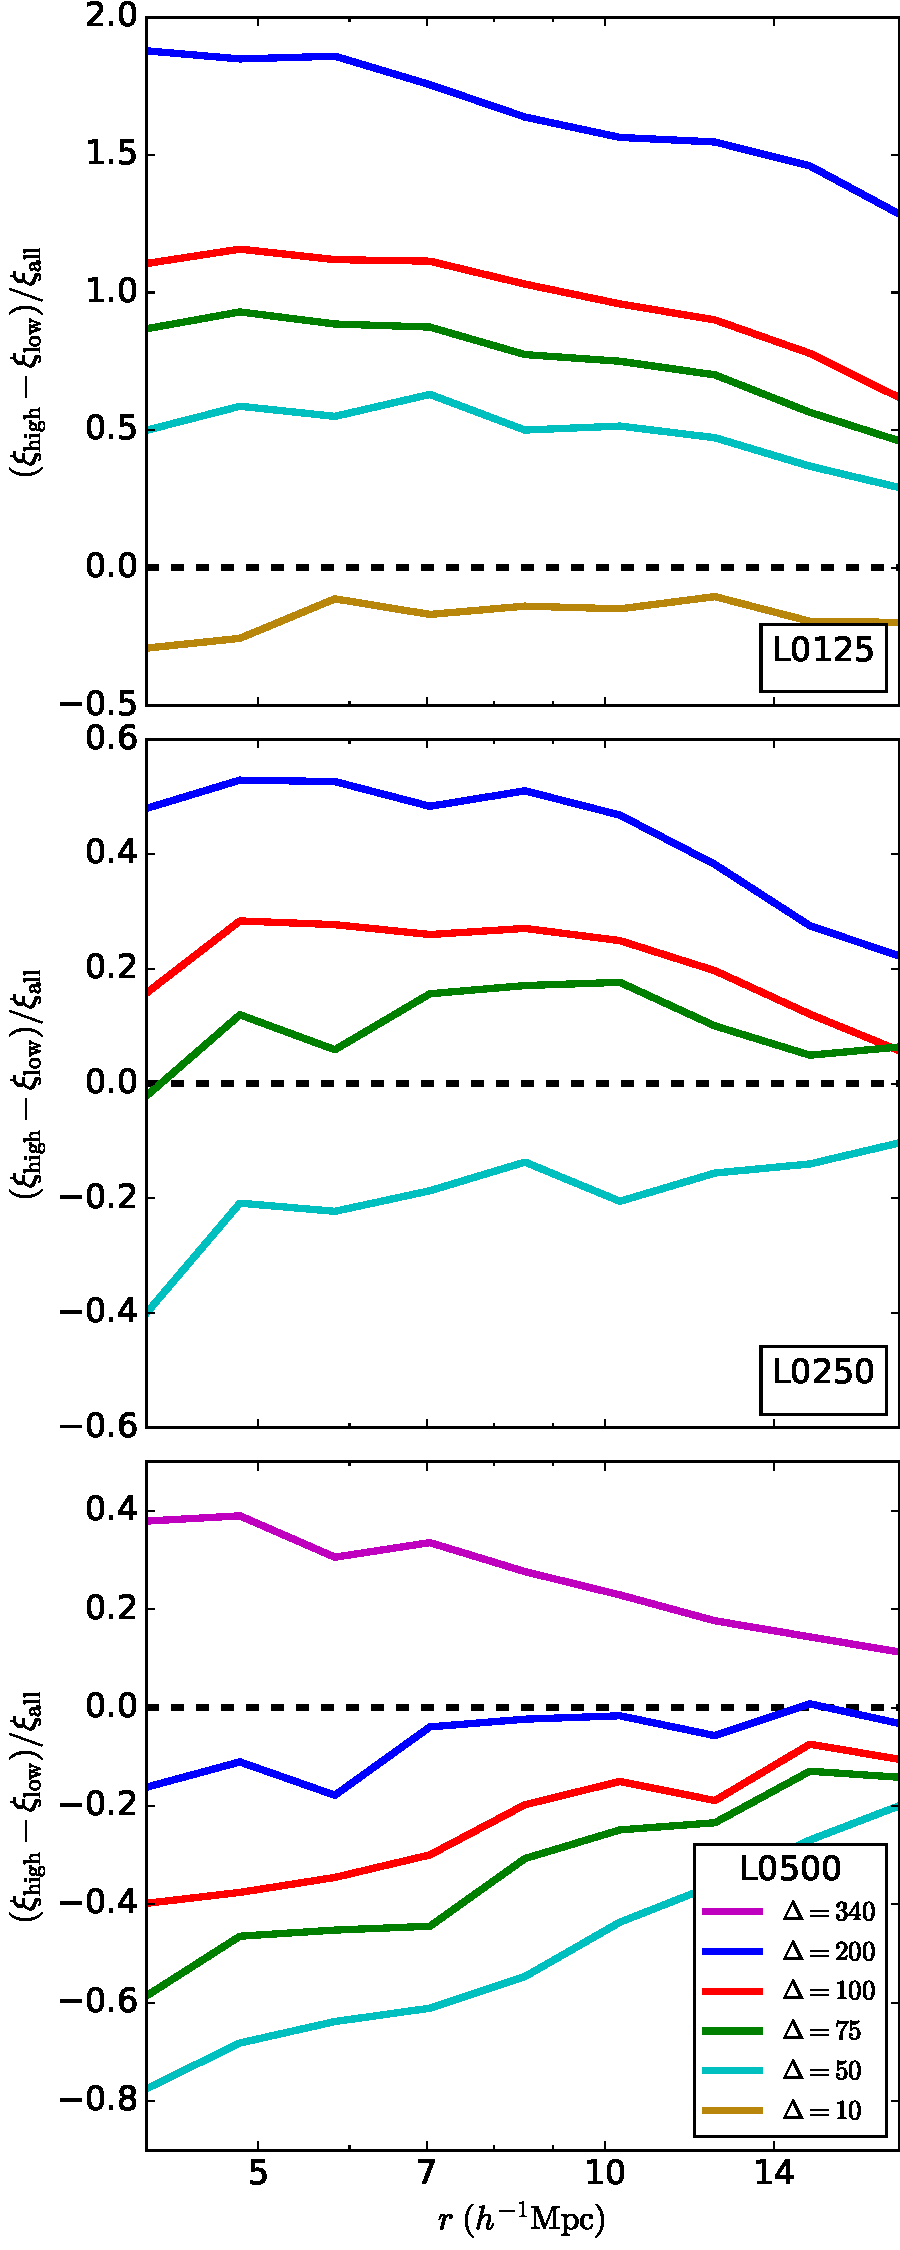
\includegraphics[width=\textwidth]{all_cfcompare_cnfw.pdf}
	\caption{
Concentration-dependent correlation functions. In each panel, the solid lines plot the difference between the correlation function for the top 20\% and the bottom 20\% of halos by NFW concentration, normalized by the correlation function of the entire halo sample. The lines correspond to different values of $\Delta$, with dark blue (light blue) corresponding to $\Delta = 625$ ($\Delta = 50$). The red dashed line in each panel  corresponds to an overdensity that greatly mitigates concentration-dependent halo clustering selected from the various values of halo overdensity that we explored. We will refer to these values throughout the text. The left (middle/right) panel shows the results for \simA \ (\simB /\simC) utilizing the low-mass (mid-mass/high-mass) halo threshold samples. The shaded bands in each panel represent the level of statistical fluctuations due to finite sampling. In particular, the shaded bands contain $98\%$ of 200 CF ratios computed from randomly subsampling halos in the $\Delta=200$ sample. In principle, each sample with a distinct $\Delta$ should have a distinct error band, but in practice they are all very similar to that of the $\Delta=200$ sample.
}
\label{fig:cc_cfcompare}
\end{figure*}
%-----------------------------------------------------------------------------------

The broad conclusions that we draw from examining CFs, such as those in Fig.~\ref{fig:cc_cfcompare} are robust to the choices we have made. For instance, we would draw the same conclusions by examining other halo subsamples (e.g., the top and bottom $10^{\rm{th}}$ percentile of halos by concentration). Furthermore, examining $c_{\mathrm{V}}$ rather than $c_{\mathrm{NFW}}$ also does not alter our general conclusions. Therefore, we do not show these additional results in the interest of brevity.

More generally, we find that for each of the halo properties that we have studied, the conclusions drawn from examining CFs are very similar to those drawn from studying MCFs. Consequently, we now move on to a more comprehensive discussion of the strength of auxiliary property-dependent halo clustering using MCFs. 

%-----------------------------------------------------------------
\subsection{Mark Correlation Functions}
\label{sub:mcfresults}

\begin{figure*}
	\centering
	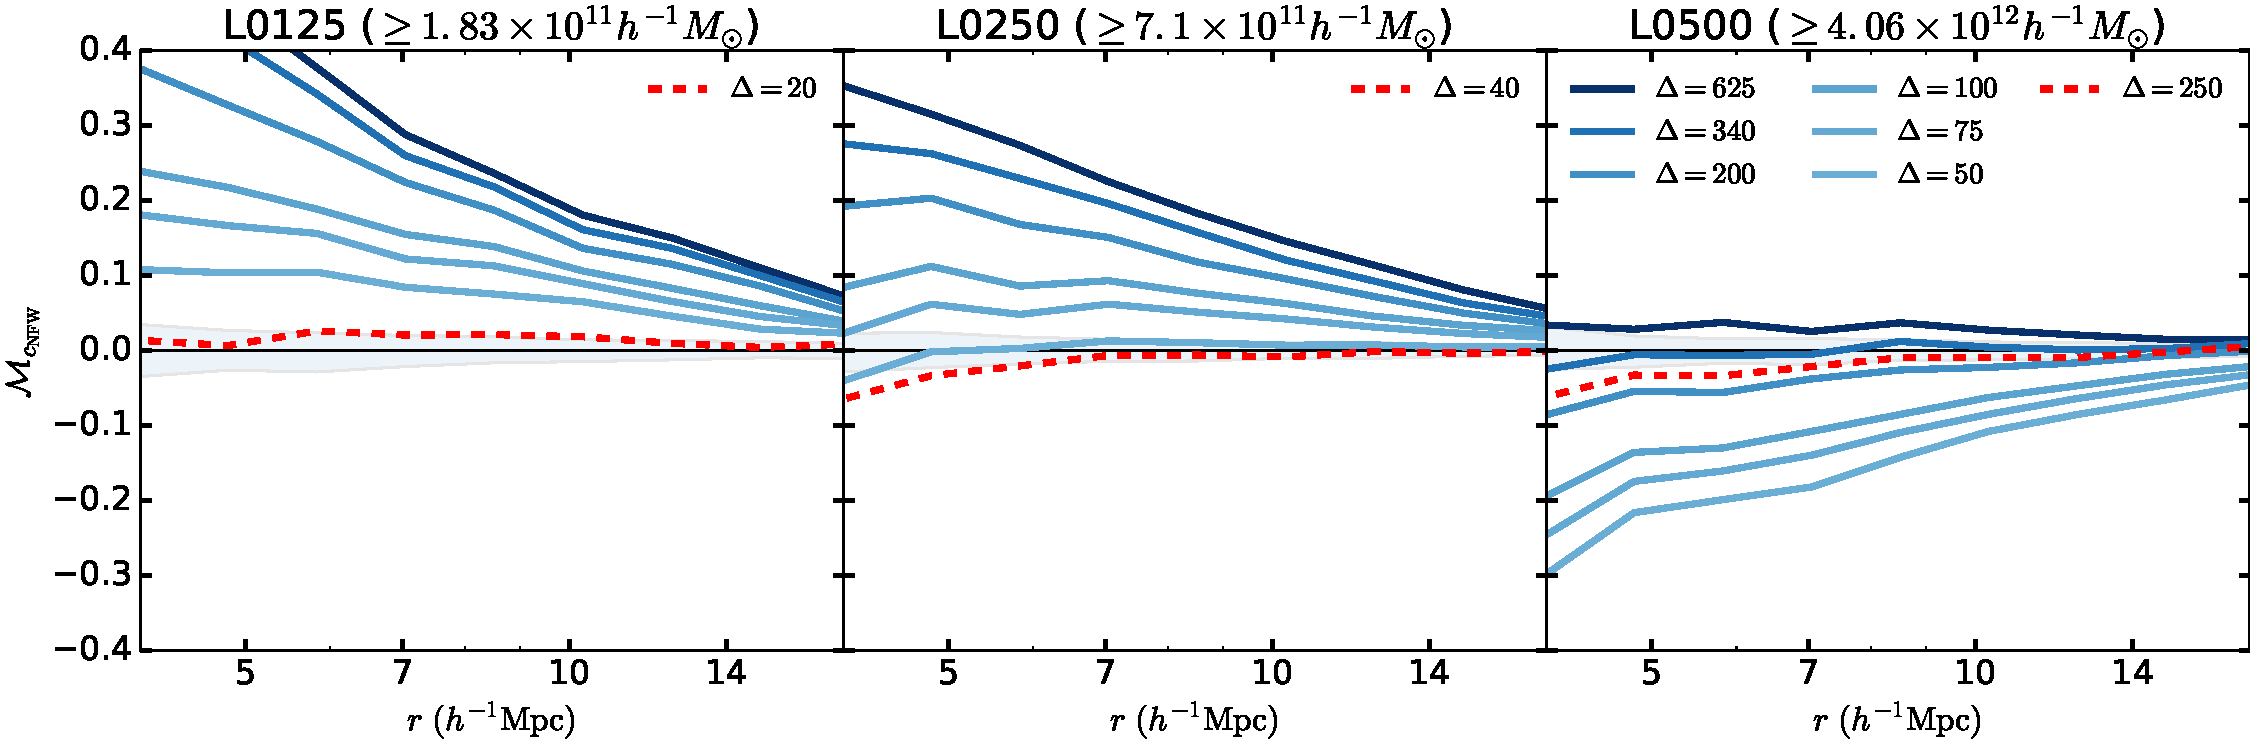
\includegraphics[width=\textwidth]{all_mcf_cNFW.pdf}
	\caption{
The marked correlation function for the concentration defined according to the NFW profile, $c_{\rm NFW}$. The solid lines plot the marked correlation function using normalized ranks of NFW concentration as the mark. In each plot the lines correspond to different values of $\Delta$, with dark blue (light blue) corresponding to $\Delta = 625$ ($\Delta = 50$). The red dashed lines correspond to the overdensities that greatly mitigate assembly bias for concentration (the same values of $\Delta$ as depicted by the red dashed lines in Fig.~\ref{fig:cc_cfcompare}). The top (middle/bottom) panel shows the results for the\simA \ (\simB /\simC) data set utilizing the low mass (mid mass/high mass) cutoffs. The shaded bands in each panel represent the level of statistical fluctuations due to finite sampling. In particular, the shaded bands contain $98\%$ of 200 MCFs computed from shuffling the halo marks among all of the halos in the $\Delta=200$ sample. In principle, each sample with a distinct $\Delta$ should have a distinct error band, but in practice they are all very similar to that of the $\Delta=200$ sample.
}
	\label{fig:cc_mcf_cnfw}
\end{figure*}


%---------------------------------------------------
\begin{figure*}
	\centering
	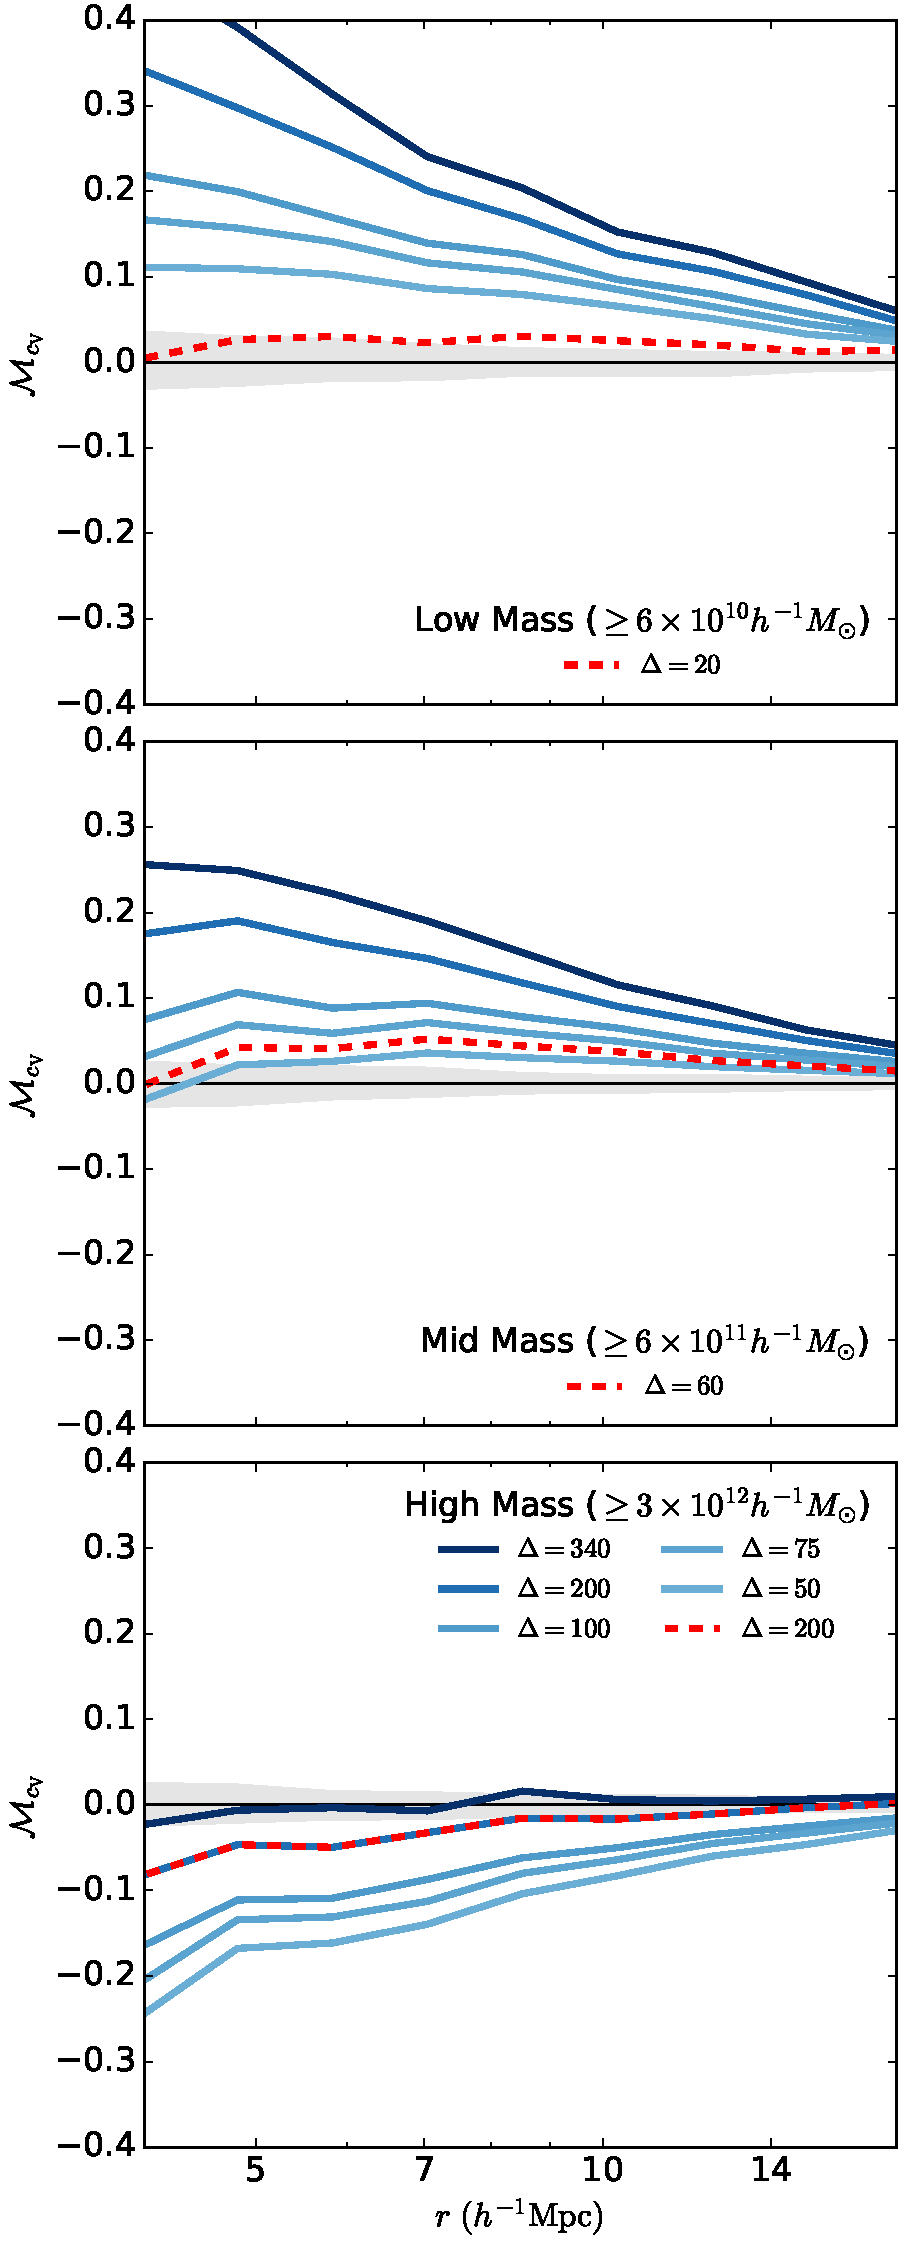
\includegraphics[width=\textwidth]{all_mcf_cV.pdf}
	\caption{	
The same as Fig.~\ref{fig:cc_mcf_cnfw} for the mark of $c_{\rm V}$.
}
	\label{fig:cc_mcf_cV}
\end{figure*}
%---------------------------------------------------



%------------------------
\subsubsection{Halo Concentration}

The NFW concentration, $c_{\mathrm{NFW}}$, MCF is shown in Figure~\ref{fig:cc_mcf_cnfw}. The shaded bands in the figure delineate the statistical fluctuations in MCFs induced by finite sampling as discussed in Section~\ref{subsection:clusteringstatistics}. In principle, each sample should be compared with a distinct band because the samples do not contain the same objects and, consequently, may exhibit different levels of statistical fluctuation. In practice, these error bands are very similar across all samples. Therefore, in Fig.~\ref{fig:cc_mcf_cnfw} and the similar plots that follow, we show only the error bands that correspond to the $\Delta=200$ halo samples. The error bands for the samples selected according to different values of the overdensity parameter are very similar and serve only to obscure the information in the figure. 

Qualitatively, Fig.~\ref{fig:cc_mcf_cnfw} exhibits the same features that are evident in Fig.~\ref{fig:cc_cfcompare}: more concentrated halos are significantly more clustered in the low-mass, L0125 halo sample; concentration-dependent halo clustering weakens and reverses sense as halo mass increases (at fixed $\Delta$), consistent with work on assembly bias \citep{wechsler_etal06,sunayama_etal16}; for the mid-mass cut L0250 sample with $\Delta=40$, the large-scale concentration dependence of halo clustering has been reduced so as to be consistent with zero within the statistical limitations of the simulation. 

Figure~\ref{fig:cc_mcf_cV} is a similar plot for the MCF of the velocity-ratio concentration, $c_{\mathrm{V}}$. This figure exhibits qualitatively very similar features to Fig.~\ref{fig:cc_mcf_cnfw}, a fact that is not surprising given that we already know that $c_{\mathrm{NFW}}$ and $c_{\mathrm{V}}$ quantify largely redundant information about their halos. This demonstrates that our results regarding the halo boundary dependence (or $\Delta$ dependence) of halo clustering is not driven by details of a fit of the density profile to the NFW functional form, which is an increasingly poor description of the halo profiles for halo-centric distances significantly great than $R_{200}$. 

%----------------------
\subsubsection{Halo Shape}

Moving on from concentrations, Figure~\ref{fig:cc_mcf_s} illustrates MCFs in which the mark is the normalized rank of the shape parameter, $s$, of the halo. For the entire range of halo masses studied, the fiducial halo definition shows that more spherical halos (those with {\em larger} marks, that is {\em larger} values of $s$) are more strongly clustered. Furthermore, Fig.~\ref{fig:cc_mcf_s} shows that increasing the sizes of halos (decreasing $\Delta$, thereby increasing the radius of the halo boundary) reduces this shape-dependent halo clustering. Unlike the case of concentration, shape-dependent halo clustering does not have a strong dependence upon halo mass.

%--------------------------------------------------- Shape MCFs
\begin{figure*}
	\centering
	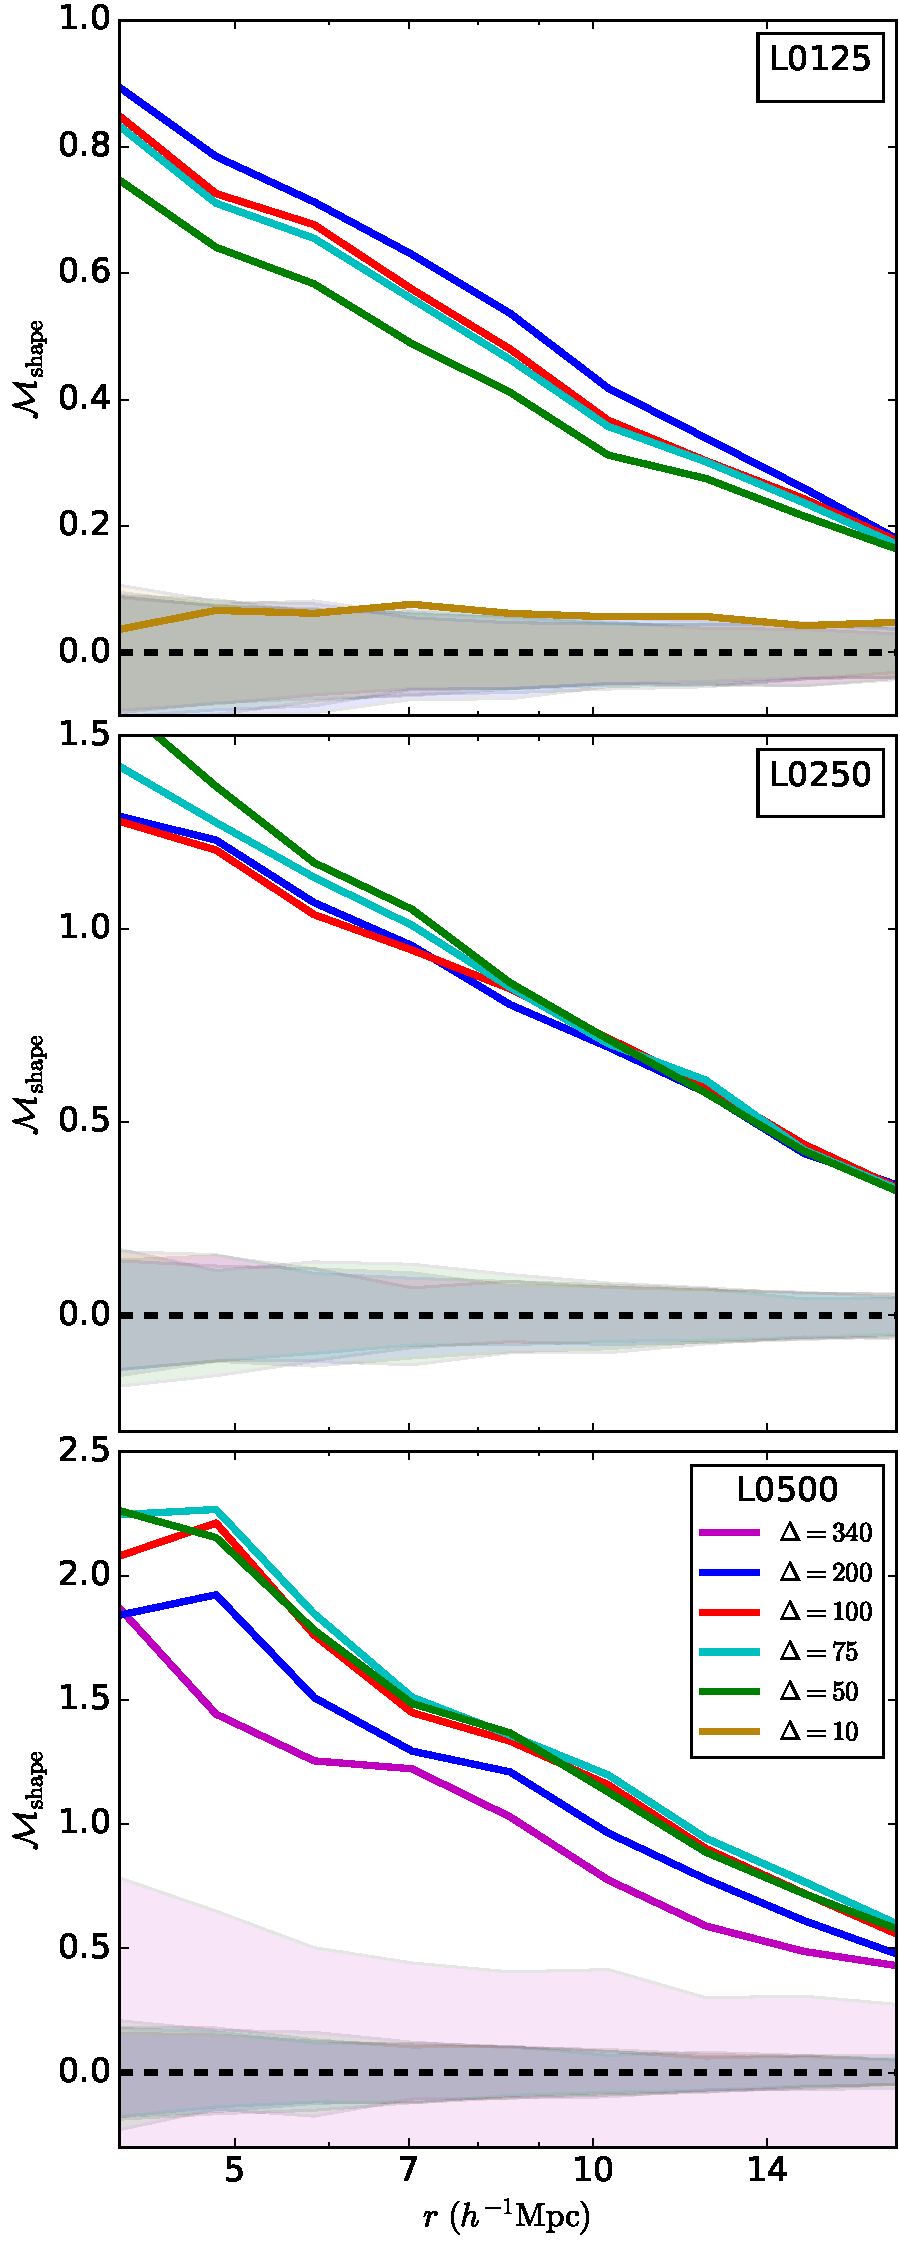
\includegraphics[width=\textwidth]{all_mcf_shape.pdf}
	\caption{
The same as Fig.~\ref{fig:cc_mcf_cnfw} for a halo shape MCF.
}
	\label{fig:cc_mcf_s}
\end{figure*}
%--------------------------------------------


Shape-dependent halo clustering also behaves differently from concentration-dependent halo clustering in that it persists even if halos are defined relative to an extremely low overdensity parameter, such as $\Delta=20$. In no case in Fig.~\ref{fig:cc_mcf_s} is shape-dependent clustering consistent with zero. No reasonable value of $\Delta$ seems to be capable of removing the enhanced clustering at the scales that we study, though the magnitude of shape-dependent clustering can be reduced by decreasing $\Delta$ (and increasing halo radii). In particular, the most effective values of $\Delta$ for removing concentration-dependent clustering, the red-dashed lines in Figure~\ref{fig:cc_mcf_s}, do not correspond with removing assembly bias from shape. 

%---------------- spin MCF
\begin{figure*}
	\centering
	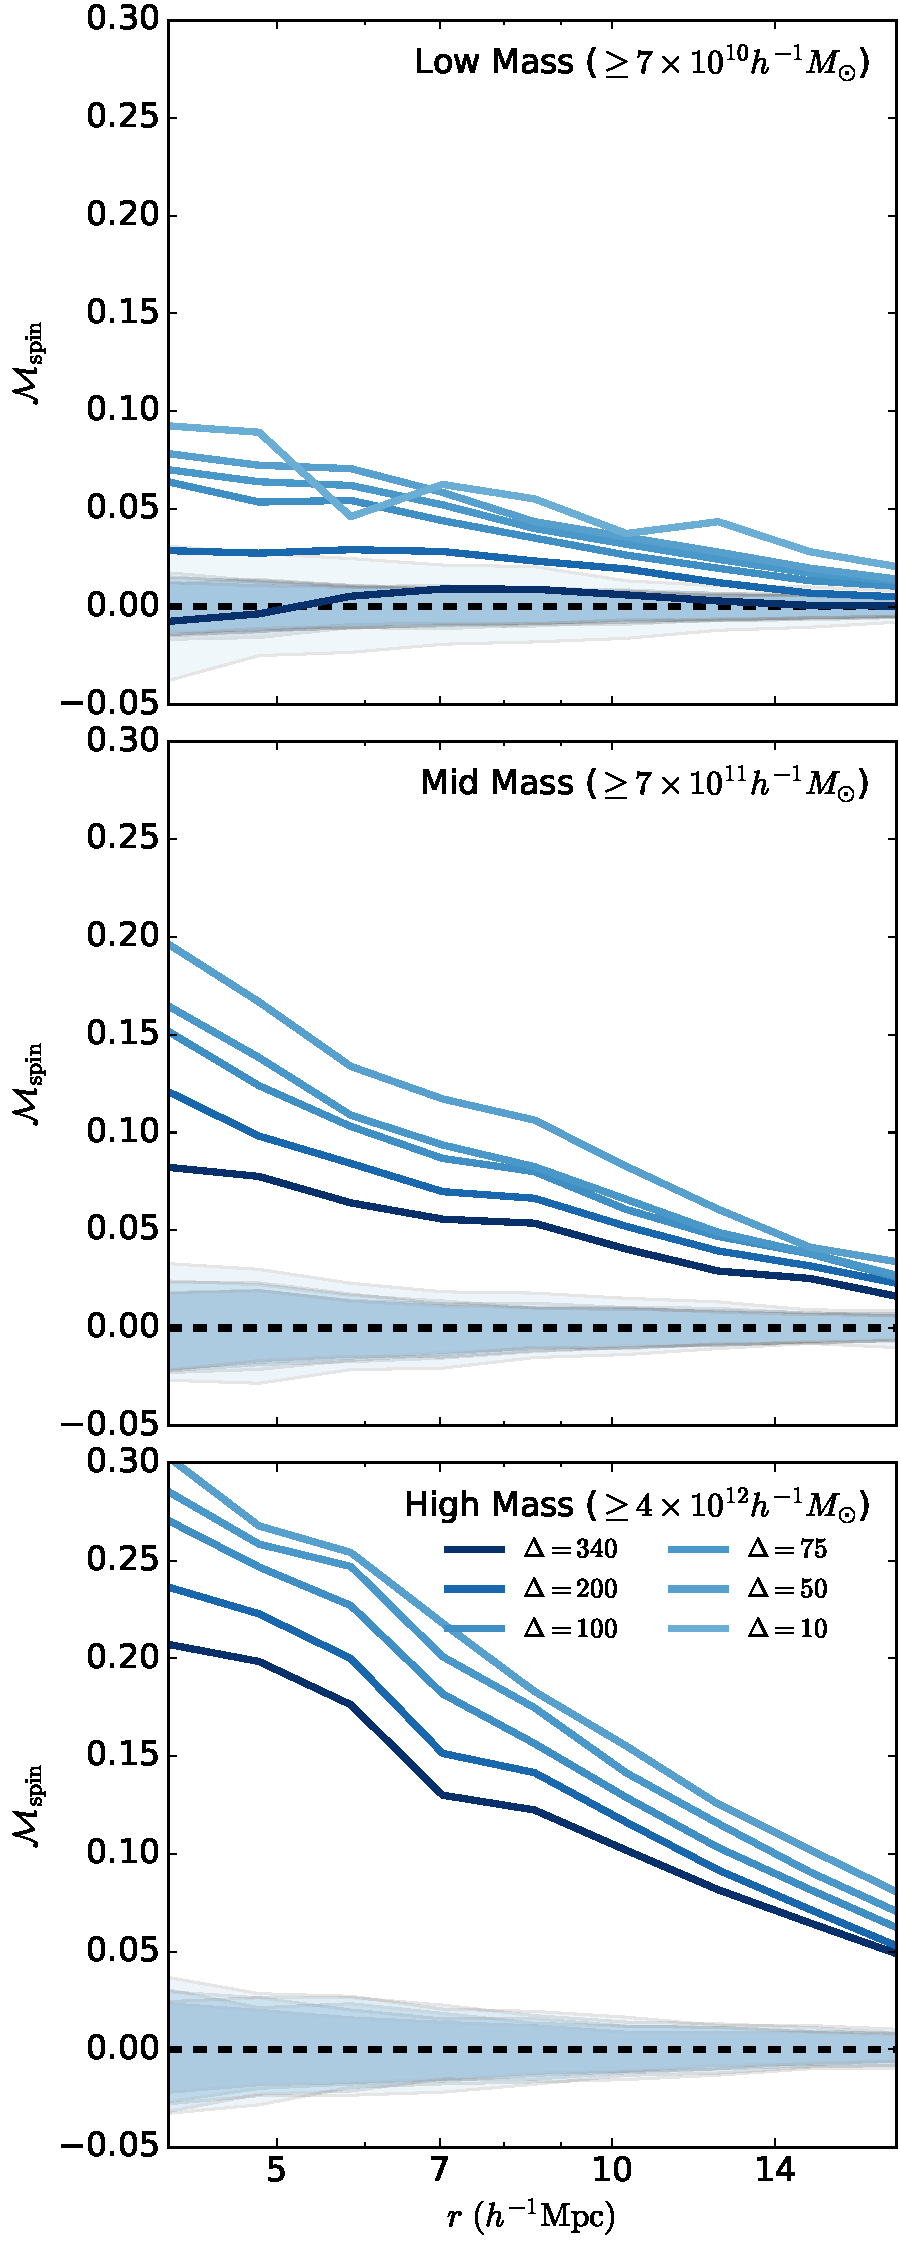
\includegraphics[width=\textwidth]{all_mcf_spin.pdf}
	\caption{
The same as Fig.~\ref{fig:cc_mcf_cnfw} for a halo spin MCF.
}
	\label{fig:cc_mcf_spin}
\end{figure*}
%-------------------------------

%------------------
\subsubsection{Halo Spin}

The spin MCFs are shown in Figure~\ref{fig:cc_mcf_spin}. In most cases, halos that are more clustered show higher values for spin than would be expected of a random sample from the one-point spin distribution, a result that is consistent with the previous literature on halo spin-dependent clustering \citep{bett_etal07,faltenbacher_white10,lacerna_padilla12}. In detail, on most scales, halos defined by overdensities of $\Delta=625$ (corresponding to an overdensity with respect to the critical density of 200) and $\Delta=340$ do not exhibit spin-dependent clustering in excess of that expected from random sampling of the spin distribution. It is also evident from Fig.~\ref{fig:cc_mcf_spin} that spin-dependent clustering is increases in strength with halo mass. For lower mass halos ($M \lesssim 7 \times 10^{11} \hMsun$ as in the mid-mass and low-mass samples) a halo definition with $\Delta \sim 625$ would yield minimal spin-dependent halo clustering; however, it is also evident that at higher masses significantly larger values of $\Delta$ would be needed to mitigate spin assembly bias\citep{hahn_etal07a,hahn_etal07b,faltenbacher_white10}

As with halo shape, it can be seen that the values of overdensity that best mitigated concentration-dependent halo assembly bias (the red-dashed lines in Figure~\ref{fig:cc_mcf_spin}) do not serve to mitigate assembly bias driven by halo spin. Indeed, halo spin exhibits a response that is qualitatively different from concentration as $\Delta$ is varied. Increasing halo radii by decreasing $\Delta$ only serves to increase the magnitude of spin-dependent assembly bias; the newly-defined halos are even more likely to have high spin if they are found in a relatively close pair with another halo. We speculate that this may be caused by material on the outskirts of halos that can carry large amounts of angular momentum with respect to the halo center (due to the large value of the impact parameter to the halo center) and that a significant amount of material contributing to angular momenta at this radii may be indicative of an overdense large-scale environment. Follow up work is necessary to determine whether or not this speculation is valid.

%----------- NFW match figure
\begin{figure*}
	\centering
	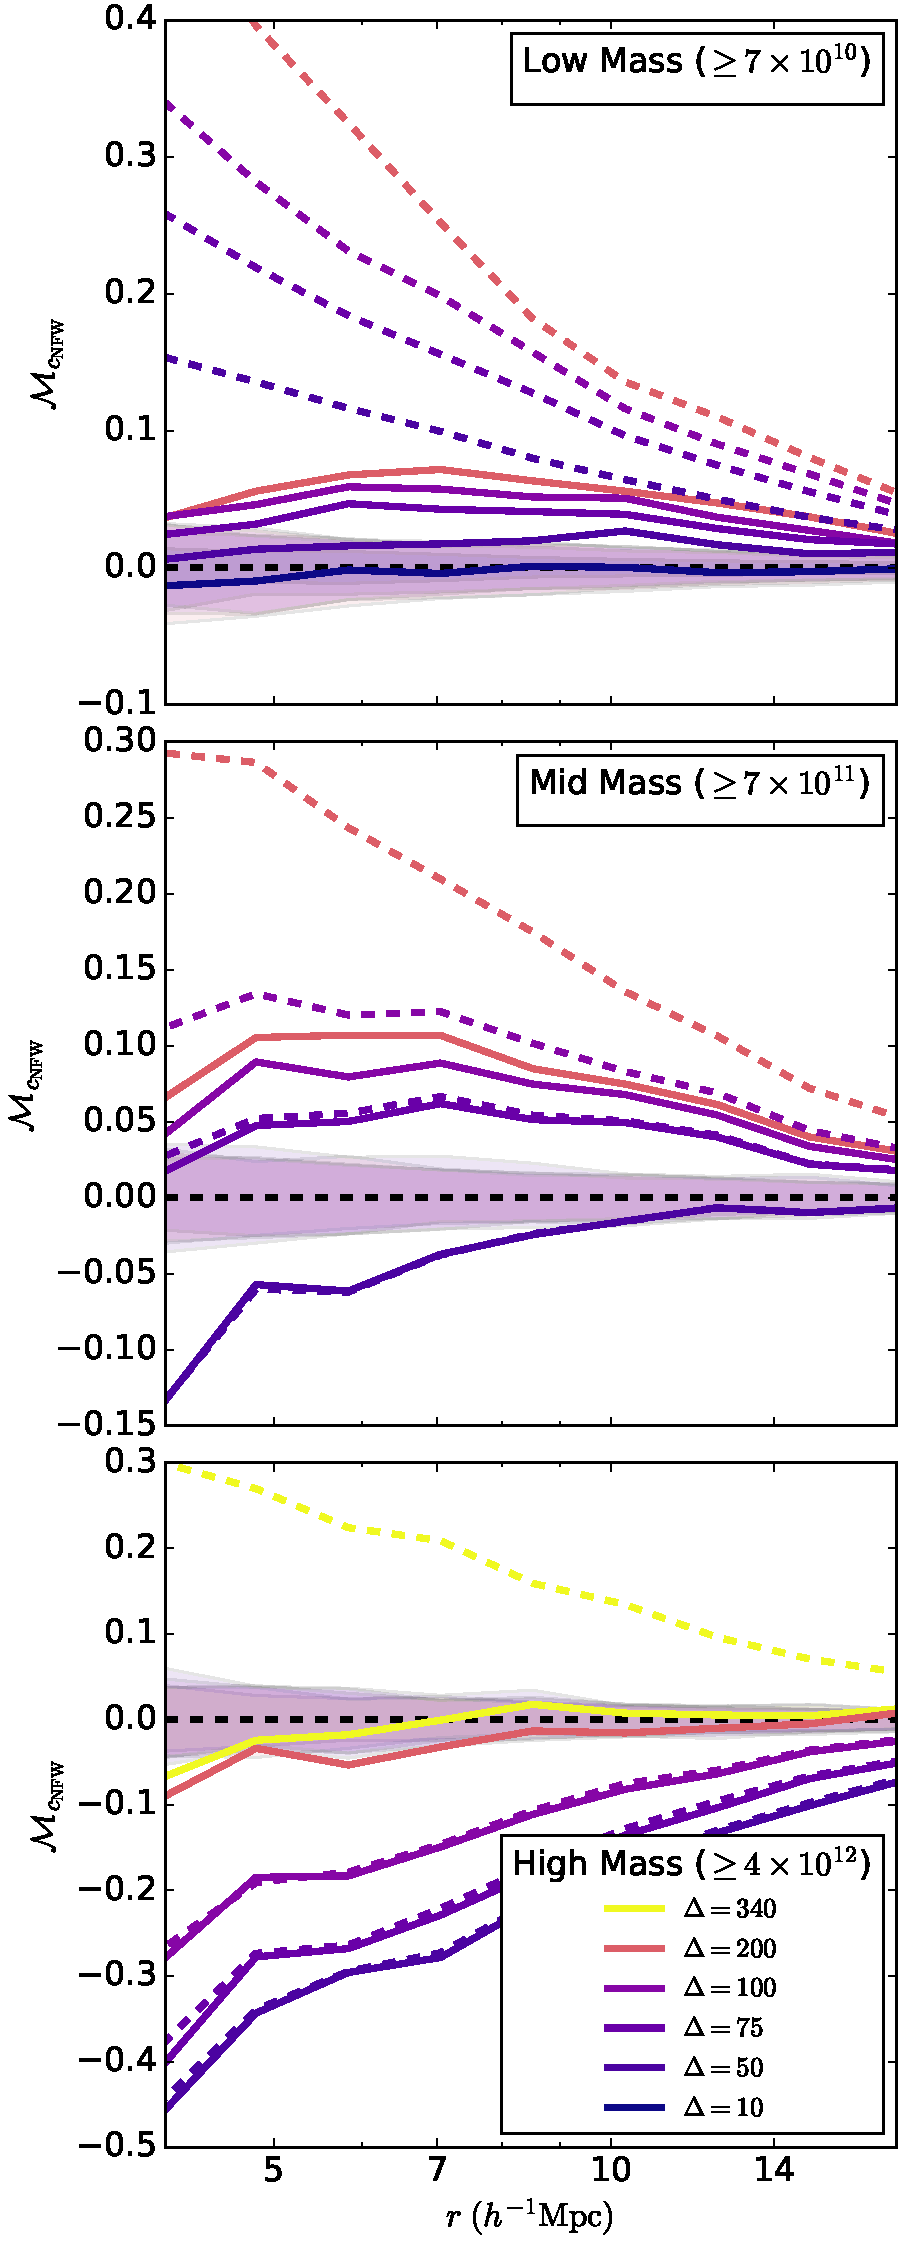
\includegraphics[width=\textwidth]{match_mcf_cNFW.pdf}
	\caption{The marked correlation function for the NFW-defined halo concentration parameter. The solid lines plot the marked correlation function using NFW-defined halo concentration as the mark, for a catalog matched against the best fit $\Delta$ shown in red. The dashed lines plot the original marked correlation function results. In each plot the lines correspond to different values of $\Delta$, with dark blue (light blue) corresponding to $\Delta = 625$ ($\Delta = 50$). The red dashed line corresponds to the overdensity chosen for matching as possibly removing assembly bias on most scales for halo concentration. The top (middle/bottom) panel shows the results for the
\simA \ (\simB /\simC) data set utilizing the low mass (mid mass/high mass) cutoffs. The shaded bands represent 2-sigma confidence regions generated by randomization of the marks. Only host halos consistent with the best-fit catalog from above are included in the analysis.\bdr{This caption describes what the figure shows, but not what it means. If I understand it correctly, this figure allows us to distinguish the different ways in which changing Delta changes assembly bias?}}
	\label{fig:hvm_mcf_cnfw}
\end{figure*}


%---Concentration-Dependent Halo Bias
\subsection{Summary of Halo Clustering as a Function of Halo Definition}

%----------------------------------------
\begin{figure*}
	\centering
	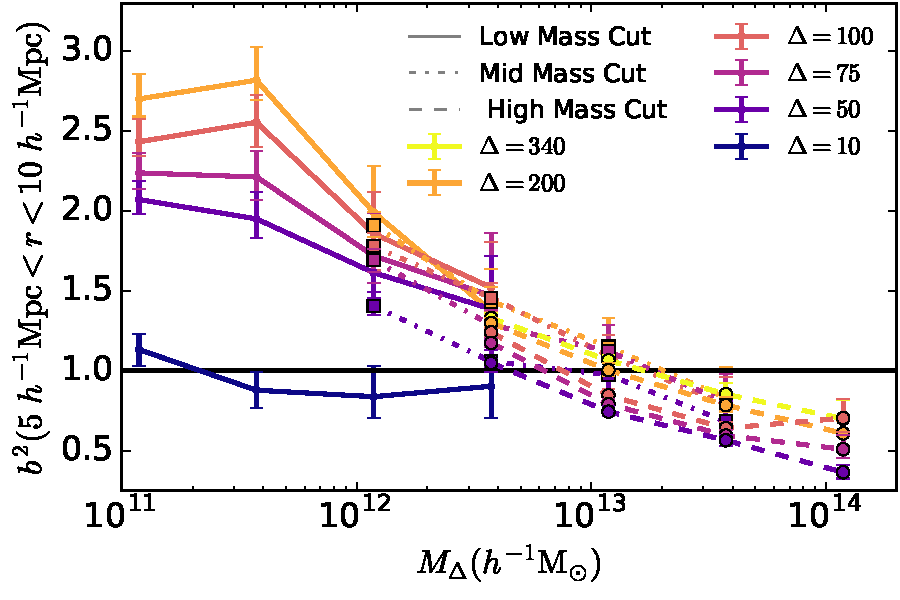
\includegraphics[width=\textwidth]{biasplot.pdf}
	\caption{
The relative clustering bias of halos as a function of halo mass for various halo auxiliary properties. For illustration in this plot, we show the clustering strength of the highest 20-percentile according to each halo property relative to the population of all halos. The properties of interest are labeled at the top of each panel. Within each panel, we show clustering biases for six values of $\Delta$. The dark blue (light blue) line uses a halo definition drawn from $\Delta = 625$ ($\Delta = 50$). The solid (dot-dashed, dashed) lines use host halos from the \simA (\simB,\simC) catalogs. The error bars on the $\Delta=200$ samples are similar to the errors from other samples, which are not shown for clarity.
}
\label{fig:biascompare}
\end{figure*}
%--------------------------------------------

Various forms of assembly bias, and their mass dependences, have already been identified in the literature. Our work confirms these previous results for halo concentrations \citep{wechsler_etal06,faltenbacher_white10,mao_etal15, sunayama_etal16}, halo shapes \citep{bett_etal07,hahn_etal07b,hahn_etal07b,faltenbacher_white10,vandaalen_etal12}, and halo angular momenta \citep{bett_etal07,hahn_etal07a,hahn_etal07b}. Our work emphasizes the fact that auxiliary property dependent halo clustering, which we refer to as assembly bias, is strongly dependent upon halo definition. 

Figure~\ref{fig:biascompare} summarizes these aspects of auxiliary property dependent clustering for each of the properties we study. Fig.~\ref{fig:biascompare} shows the {\em relative} halo clustering bias of high-$p$ halos, where $p$ is the property of interest, compared to all halos defined as: 
\beq
b^2(r) = \xi_{p,80\%} / \xi_{\mathrm{all}},
\eeq
%
where $\xi_{p,80\%}$ designates the clustering of halos in the $80^{\mathrm{th}}$ percentile of $p$ at fixed mass (that is, the halos with the $20\%$ highest $p$ values). To summarize clustering strength with a single relative bias, we computed pair counts within a wide bin of separations from $5-10\, \hMpc$. The wide bin width is justified partly by the mild scale dependence shown in Fig.~\ref{fig:cc_cfcompare}. We estimated the errors on the relative bias by recomputing $\xi_{\mathrm{all}}$ using randomly-selected subsamples of equal number to the subsample used to compute $\xi_{p,80\%}$, that is, using one fifth of all halos. The error bars show the $68\%$ range, centered on the median, 
about which the values of $b^2(r)$ lie. 

Each panel of Fig.~\ref{fig:biascompare} allows us to focus on the mass dependence of halo clustering and the dependence on halo definition. Focus first on the top two panels, which deal with our two halo concentration measurements, NFW concentration and velocity ratio concentration. Both measures of concentration exhibit a strong mass dependence to assembly bias. Halos at high masses ($M_{\Delta} \ge 10\times10^{13}$) exhibit minimal assembly bias compared to those at low masses ($M_{\Delta} \le 10\times10^{12}$). 

Concentration dependent halo clustering also shows a significant dependence upon halo definition. In particular, the strength of clustering of the halos above the $80^{\rm{th}}$ percentile in concentration varies by as much as $\sim 50\%$ among the overdensities that we have investigated. For all halo definitions, 
the concentration-dependent clustering exhibits a similar trend with halo mass. For no value of $\Delta$ does the trend with mass become significantly less prominent, suggesting that a simple re-definition of halo boundaries alone cannot eliminate halo assembly bias. Concentration-dependent clustering changes sense at a mass that varies by order of magnitude, from $\sim 3 \times 10^{12}\, \hMsun$ to $\sim 3 \times 10^{13}\, \hMsun$, as $\Delta$ varies from $\Delta=50$ to $\Delta=625$. These significant variations in the strength of concentration-dependent clustering as a function of halo definition suggest that significant care must be taken in comparisons of various results in the extant literature.

The bottom two panels of Fig.~\ref{fig:biascompare} demonstrate that auxiliary property dependent clustering can behave in a markedly different manner depending upon the halo property under consideration. These two panels show shape (left) and spin (right) dependent clustering as a function of halo mass and halo definition ($\Delta$). Each demonstrates halo assembly bias that is only weakly dependent on halo mass at the scales we have analysed. In the lower-left panel, note that changing to smaller values of $\Delta$ results in reduced assembly bias, though no definition explored was sufficient to remove assembly bias entirely. 

%---------------------------------------------------------------------------------------------
\section{Discussion}
\label{section:discussion}
%---------------------------------------------------------------------------------------------

%----------------------------
\subsection{Broad Conclusions}
%----------------------------

We have studied the clustering of dark matter halos as a function of halo properties other than mass. We have confirmed that for conventional halo definitions halo clustering strength is a strong function of the  ``auxiliary properties'' that we studied, namely halo concentration (either measured through a fit to the NFW profile or assigned non-parametrically as the ratio of the maximum circular velocity to the virial velocity), halo shape, and halo spin. These findings are consistent with the now significant literature on the subject subject of halo assembly bias. \citep{peacock_smith00, wechsler_etal02,sheth_tormen04, gao_etal05, zentner_etal05, allgood_etal06, harker_etal06, wechsler_etal06, croton_etal07, zentner07, dalal_etal08, zentner_etal14, mao_etal15, sunayama_etal16}

We have explored auxiliary property dependent halo clustering as a function of halo definition, parameterized by overdensity parameter $\Delta$. This exploration was motivated, in part, to determine whether alternative halo definitions can mitigate the dependence of halo clustering on these ``auxiliary properties.'' We find that these alternative halo definitions do {\em not} generally mitigate the effects of assembly bias. We are led to this conclusion for two reasons. First, no single halo definition serves to mitigate auxiliary property dependent clustering for all of the auxiliary properties that we have investigated. Indeed, modified halo definitions, with low values of $\Delta$, may lead to stronger auxiliary property dependent clustering as is the case with halo spin, for example.

Second, the halo definitions that mitigate assembly bias are strongly halo mass dependent. In the case of halo concentration, which we examine in the most detail, assembly bias is strongly mitigated for halo definitions of $\Delta \approx 20$, $\Delta \approx 40$, and $\Delta \approx 250$ for halos in our $M \geq 1.83 \times 10^{11} \hMsun$, $M \geq 7.1 \times 10^{11} \hMsun$, and $M \geq 4.06 \times 10^{12} \hMsun$ mass threshold samples respectively. Of course, this mass dependence may not be surprising given the well-known mass dependence of assembly bias. Physically, this is likely due to the fact that concentration-driven assembly bias may be caused by distinct mechanisms at the low-mass and high-mass end of the halo mass spectrum \citep[e.g., see][]{zentner07,wang_etal07,dalal_etal08}. 

The two observations together suggest that it may well be possible to mitigate assembly bias for a single halo property (e.g., concentration) by using a mass-dependent halo definition. However, this mass dependence will render the halo definition quite complex. We discuss the particular case of concentration-dependent clustering further below.

Our work emphasizes the important dependence of halo assembly bias upon halo definition, which is not yet widely appreciated. In each of Figures \ref{fig:cc_mcf_cnfw} through \ref{fig:cc_mcf_spin}, the strength of assembly bias is a strong function of halo definition. This definition dependence is not restricted to extreme choices of the overdensity parameter $\Delta$. The difference in the strength of assembly bias between a ``virial'' halo definition, with $\Delta=340$, and a definition with $\Delta=200$ is considerable. Likewise, defining halos using an overdensity of 200 relative to the critical density, corresponding roughly to $\Delta \approx 625$ in our notation, also leads to significant, quantitative differences in the strength of assembly bias. Indeed, distinct halo definitions may even lead to assembly bias of opposite sense. For example, at fixed halo mass, higher concentration halos may be more strongly clustered by one halo definition and more weakly clustered by another. It is interesting to consider that some of the variety of results pertaining to the strength of assembly bias in the literature may be partly induced by the different halo definitions used by different authors.

%-------------------------------------------
\begin{figure*}
	\centering
	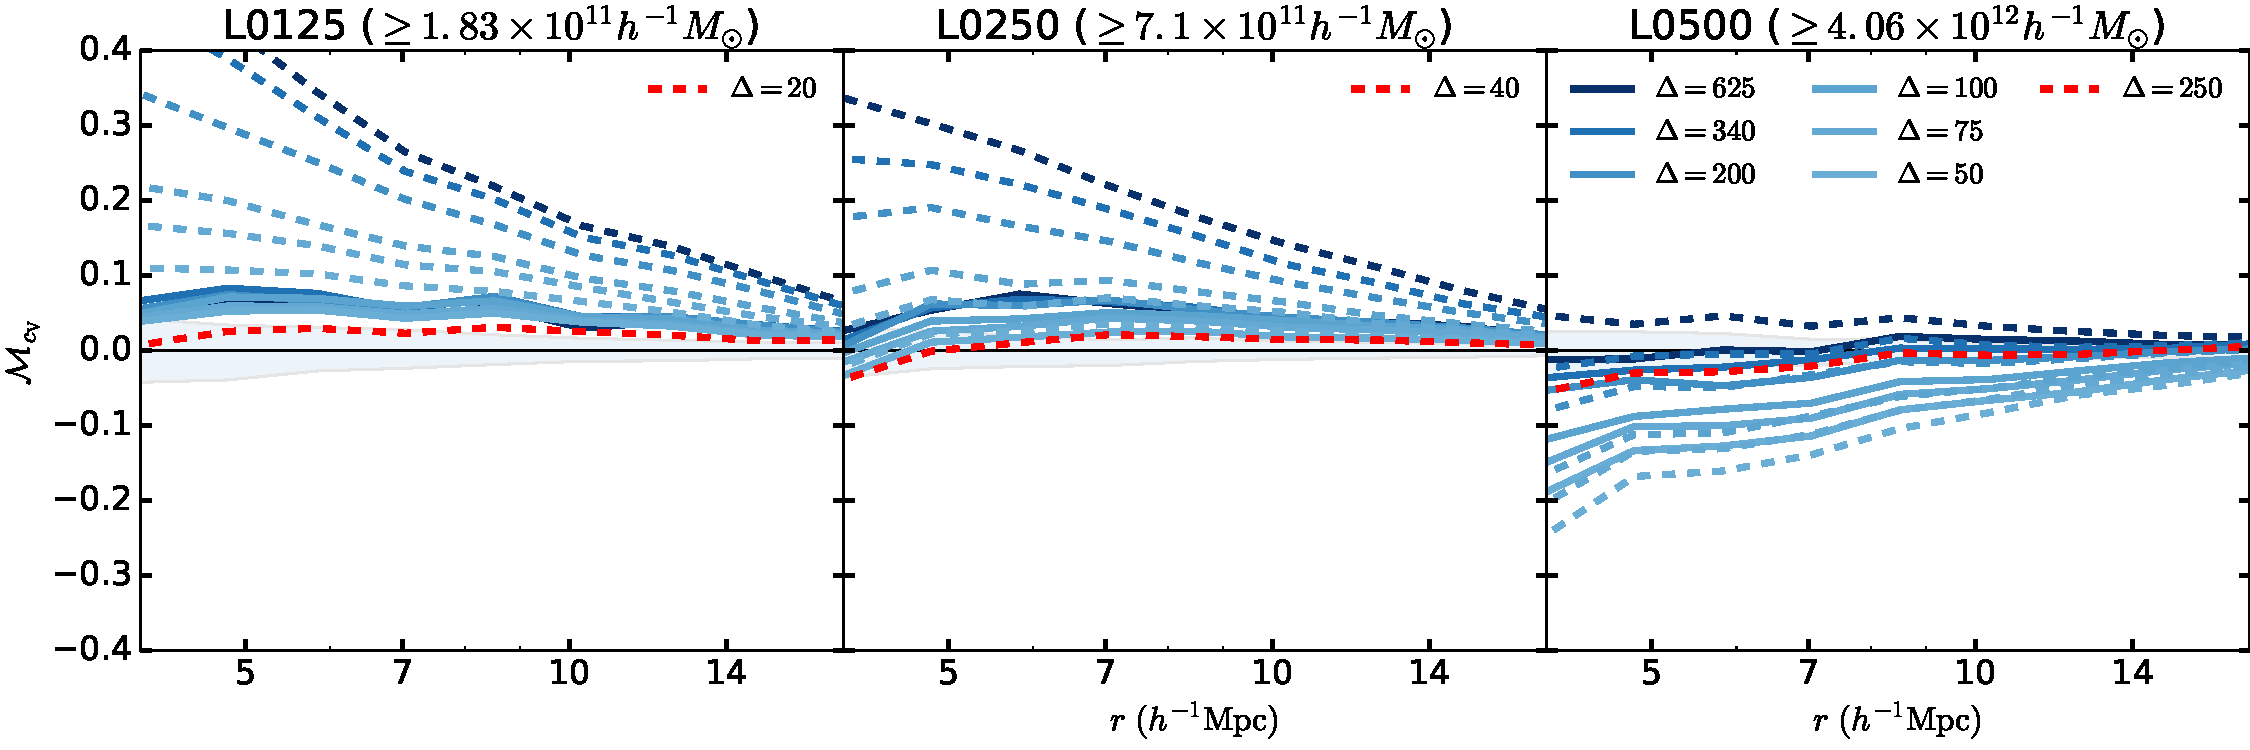
\includegraphics[width=\textwidth]{match_mcf_cV.pdf}
	\caption{As Fig.~\ref{fig:hvm_mcf_cnfw}, with the mark defined as velocity ratio defined concentration.
}
	\label{fig:hvm_mcf_cV}
\end{figure*}
%-----------------------------------------------

%------------------------------------------------
\subsection{How Does Halo Definition Mitigate Concentration-Dependent Halo Clustering}
%------------------------------------------------

As mentioned above, our results indicate that one may mitigate auxiliary 
property dependent clustering through a mass-dependent choice of halo 
definition. It is interesting to ask why halo redefinitions may be 
helpful. In this subsection, we discuss the particular case of halo 
concentration dependent clustering in more detail in part because 
concentrations may be the most physically interesting property that 
we have studied.

Halo redefinitions may mitigate concentration-dependent halo bias for at least two reasons. The first reason and physical motivation for exploring halo alternative halo definitions is that alternative definitions may identify regions with halos in a more practically useful manner. In particular, larger halo definitions (lower $\Delta$) may incorporate objects that have been strongly affected by nonlinear evolution into a single halo. In such a case, halo redefinition is physically motivated and may constitute a pragmatic step forward. However, alternative halo definitions may reduce auxiliary property dependent clustering a second way. In particular, it is possible that the details of measuring halo properties using these new halo definitions introduce new sources of noise into the measurements. The inherently noisier measurements then lead to reduced correlations. In this second case, the reduction in correlations arises because the property of interest may be {\em less} informative about the halo itself.

For the case of halo concentration, noise may be introduced in numerous ways. For example, the NFW concentration $c_{\mathrm{NFW}}$ is determined by a fit to the 
NFW profile. Inferred values of $c_{\mathrm{NFW}}$ will depend upon 
the degree to which the density profiles of the halos follow the NFW 
functional form within some radius $R_{\Delta}$ that is different from 
traditional halo radii, such as $\sim R_{200}$. At large halocentric 
distances ($r \gtrsim R_{200}$) halo profiles are known to deviate 
from the NFW form. It may be possible to reduce assembly bias by redefinitions if one probes scales on which halos deviate from NFW in a way that is not well correlated with the interior structure of the halo (particularly the location of the NFW scale radius); however, such a reduction in assembly bias is of limited practicality because it arises from characterizing a halo by a quantity that is less informative about its interior structure. Of course, it is worth noting that the velocity-defined concentration $c_{\rm V}$ is a non-parametric measure of concentration and should be less subject to such effects. 

We can explore in more detail the degree to which the mitigation of environmental effects by halo redefinition are due to introducing noise that is uncorrelated with environment into the measurement of halo properties. We proceed as follows. All host halos that are found in the halo catalogs constructed from lower values of $\Delta$ (e.g., $\Delta=40$) are also present as host halos in the halo catalogs constructed with all higher values of threshold density (e.g., $\Delta=200>40$). The converse is not true because lowering $\Delta$ increases halo radii so that host halos at higher values of $\Delta$ may become subhalos at lower values of $\Delta$\footnote{Indeed, this is largely the motivation for exploring various $\Delta$.}. Therefore, we consider the clustering of only those host halos that exist in a higher $\Delta$ catalog as well as a lower $\Delta$ catalog. An example may help to clarify our procedure. Consider the clustering of the subset of host halos identified within the the $\Delta=200$ catalog (and with all properties assigned to a conventional $\Delta=200$ halo), that also exist within a $\Delta=40$ catalog. Those host halos that {\em do not} exist in the $\Delta=40$ catalog are precisely those halos that have been subsumed by the larger halo radii in this case and thus been classified as subhalos. This achieves the goal of redefining halos by the lower $\Delta$ threshold ($\Delta=40$ in this example), but eliminates the possibility that the properties we are studying are also defined differently in the lower $\Delta$ catalog, because we are studying their clustering as a function of the properties defined in the higher $\Delta$ ($\Delta=200$ in this example) catalog. We refer to samples constructed in this way as ``matched'' halo samples between two values of threshold overdensity $\Delta$. 


The dashed lines in Figure~\ref{fig:hvm_mcf_cnfw} show the same MCFs depicted 
in Fig.~\ref{fig:cc_mcf_cnfw}. The solid lines in Fig.~\ref{fig:hvm_mcf_cnfw} show MCFs for halo samples in ``matched'' halo catalogs in which the lower $\Delta$ is indicated in each panel (and depicted by the red, dashed lines). These lower 
values of $\Delta$ are chosen effectively to remove assembly bias at large scales based on the results in Fig.~\ref{fig:cc_mcf_cnfw}, 
$\Delta=20$ for the \simA~ cut, 
$\Delta=40$ for the \simB~ cut, 
and $\Delta=250$ for the \simC~ cut. 


In comparing a pair of dashed and solid lines at the same $\Delta$ threshold in Fig.~\ref{fig:hvm_mcf_cnfw}, one is comparing the MCF of all halos at that $\Delta$ threshold, to the MCF of only those halos identified in the lower threshold samples. The difference between a pair of solid and dashed lines at fixed $\Delta$ is caused entirely by the exclusion of some halos from the lower $\Delta$ catalog due to a change in halo definition. Notice that the solid lines exhibit greatly reduced concentration-dependent clustering. Selecting particular halos as hosts eliminates a large contribution to concentration-dependent clustering. Fig.~\ref{fig:hvm_mcf_cV} displays analogous results for the velocity-defined concentration parameter $c_{\rm V}$. These results suggest that much of concentration-dependent clustering is driven by the interactions of nearby halos. They also suggest that subsuming larger regions into halo definitions to accommodate these interactions may be well motivated and practically useful in the context of halo occupation models. It may even be possible to optimize halo definitions for specific applications. 

In each panel in Fig.~\ref{fig:hvm_mcf_cnfw}, there is some modest residual assembly bias displayed by the solid lines; the solid lines are not all consistent with zero. This suggests that redefining halos with larger radii (smaller $\Delta$) may, in part, reduce assembly bias through the introduction of noise in the concentration measurement, rendering it less informative about the interior structure of the halo. Nonetheless, this residual assembly bias is generally modest compared with the concentration-dependent clustering of halos defined with more traditional values of overdensity threshold.

%---- Splashback Comparison
\subsection{Halo Definitions and the Splashback Radius}

Our study is reminscent of, and indeed motivated by, much of the recent work on halo splashback radii \citep{more_etal15,mansfield_etal16,diemer_etal17}. Briefly, the splashback radius of a halo is intended to be the halo-centric distance that characterizes the orbital apocenters of accreted halo material. It is, therefore, a well motivated criterion for separating the halo region, within which halo interactions are clearly important, from larger scales, where halo interactions may be less important. Our perspective is to generalize this idea by identifying the importance of interactions by investigating the environment dependence of halo properties themselves (e.g., halo concentrations). Consequently, it is interesting to compare our results with halo splashback radii. 

In Figure~\ref{fig:splashback_compare}, we show a first, broad comparison of our work with halo splashback radii. The blue points in Fig.~\ref{fig:splashback_compare} show the radii (in units of the traditional $R_{200}$ halo radius) of halos selected at each of the $\Delta$ thresholds that minimize concentration dependent halo clustering as a function of halo mass $M_{200}$. As we have already remarked, our work suggests that halo definition must be a rapidly varying function of halo mass in order to mitigate assembly bias. The red line depicts the mean halo splashback radii of halos of fixed mass as a function of $M_{200}$ \citep{diemer_etal17}. Clearly, our results suggest that identification of halos using splashback radii alone will not greatly mitigate assembly bias. 

%-------------- splashback comparison --
\begin{figure}
	\centering
	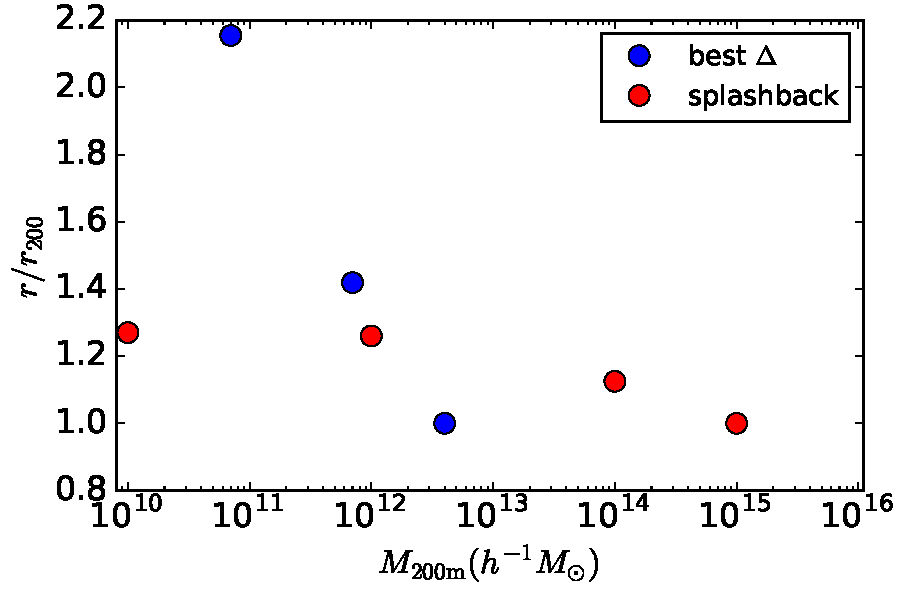
\includegraphics[width=\columnwidth]{test_splashback.pdf}
	\caption{A comparison of the average ratio between $r_{200}$ and the splashback radius as determined by \citet{diemer_etal17} (red line) to the average ratio between $r_{200}$ and the halo radius determined as our best choice of $\Delta$ for removal of assembly bias as discussed above (blue circles). There is some dispersion in $R_{\Delta}$ but it is quite small (see Fig.~\ref{fig:deltacompare}) so we do not show it on the blue points. Note that the halo mass chosen for the blue points is determined by the mass cutoff in the simulation analysis, as the smallest (and most numerous) halos dominate the calculation. 
}
	\label{fig:splashback_compare}
\end{figure}
%---------------------------------------

%----------------------
\section[]{Conclusions}
\label{section:conclusions}
%----------------------

We have examined the dependence of halo assembly bias upon halo definition, parameterized, for simplicity, by spherical overdensity threshold $\Delta$. 
This work was motivated as an effort to determine whether not not the 
dependence of halo clustering strength on halo properties other than mass 
could be mitigated by judicious choice of halo definition. In concluding this study, we 
draw the attention of the reader to the following conclusions.

\begin{itemize}
    
  	\item The degree to which halo clustering depends upon auxiliary halo properties varies considerably with halo definition. This is particularly true of halo concentration. 
    
    \item A judicious definition of a halo can greatly mitigate concentration-dependent halo clustering. However, this requires a halo definition that has a strong mass dependence; a threshold of $\Delta=20$ mitigates assembly bias at low masses 
($M_{200} \sim 1.8 \times 10^{11}\, \hMsun$) but induces assembly bias of opposite sense at high masses 
($M_{200} \gtrsim 4 \times 10^{12}\, \hMsun$). 
At high masses 
($M_{200} \gtrsim 4 \times 10^{12}\, \hMsun$) 
an overdensity of $\Delta \approx 340$ results in 
very weak concentration-dependent clustering. 
    
    \item Halo shape requires an extreme halo definition, $\Delta \sim 10$ in order to mitigate shape-dependent clustering.
    
    \item Halo spin dependent clustering demonstrates assembly bias that increases with halo mass. Spin-dependent assembly bias can be mitigated with a threshold of 
$\Delta \sim 340-625$ for the lowest masses ($M_{200} \sim 1.8 \times10^{11}\, \hMsun$), while considerably larger values of $\Delta$ must be used at higher masses 
($M_{200} \gtrsim 4 \times 10^{12}\, \hMsun$). 

    \item Although our study was motivated, in part, by recent studies of the ``splashback radius,'' there is no clear connection between our preferred halo definitions and halo spashback radii. This is shown in Fig.~\ref{fig:splashback_compare}. More detailed explorations await future work.
    
    \item We summarize many of our results in Fig.~\ref{fig:biascompare}, which gives an example of the mass and halo definition ($\Delta$) dependence of the strength of halo assembly bias.
    
\end{itemize}

These conclusions are strongly suggestive of the fact that choosing to model halos with a single common definition of halo size from overdensities requires extensive modelling to mitigate the impact of assembly bias. It is possible that there are halo properties that are impacted less than those that we studied in this work: a thorough examination of other potential properties may merit further analysis.

It is worth noting that one difference between the approach utilized in the splashback radii approach \citep{more_etal15,diemer_etal17} and our halo redefinition approach outlined in this work. The identification of splashback radius is done on a halo-by-halo basis to try to identify a physically meaningful substructure. Though beyond the scope of this work, this might well bear similarities to choosing the best value of $\Delta$ on a halo-by-halo basis, rather than as a single value for the entire mass range. We hope to explore the effect of splashback radius with similar analysis in future work.

\arz{Antonio, I removed the last two paragraphs here. They don't seem to be saying anything. If you want to write a punchy final paragraph or two, give it a shot.}
\asv{I think a key thing to draw from the conclusions is that a single bulk halo definition is unlikely to mitigate assembly bias. I tried to suggest as much here (linking again back to splashback radius approaches), but I am uncertain if this feels out of place with the narrative or if there is a better way to word this.}

\section*{Acknowledgements}

We are grateful to many people. Our calculations are carried out utilizing the
{\tt numpy} \citep{numpy}, {\tt astropy} \citep{astropy}, {\tt matplotlib} 
\citep{matplotlib}, {\tt colossus} \citep{diemer_kravtsov15}, and {\tt halotools} \citep{halotools} packages in Python. The work of ASV and ARZ has been supported, in part, by grants AST 1516266 and AST 1517563 from the U.S. National Science Foundation (NSF) as well as by the Pittsburgh Particle physics, Astrophysics, and Cosmology Center (Pitt PACC) at the University of Pittsburgh. KW is supported by NSF grant AST 1517563. YYM is supported by the Langley Fellowship at Pitt PACC. CWP is supported by BLAH. APH is supported by BLAH. FCvdB is supported by BLAH. BD is supported by BLAH. JUL is supported by BLAH. 

\bibliographystyle{mnras}
\bibliography{master}

\label{lastpage}

\end{document}
